\documentclass[a4paper,12pt]{report}

\usepackage[utf8]{inputenc}
\usepackage[T1]{fontenc}
\usepackage[turkish]{babel}
\usepackage{setspace}
\usepackage{geometry}
\usepackage{graphicx}
\usepackage{amsmath}
\usepackage{url}

\geometry{margin=3cm}
\onehalfspacing

\begin{document}

\begin{titlepage}
\begin{center}

\vspace*{1cm}

% ===== TOP OF PAGE =====
{\Large \textbf{PAMUKKALE ÜNİVERSİTESİ}}\\[0.3cm]
{\large \textbf{Mühendislik Fakültesi}}\\[2cm]

% ===== TITLE =====
{\Large \textbf{AURA FINANCE: YAPAY ZEKÂ DESTEKLİ VE HİBRİT BÜTÇE OPTİMİZASYONLU KİŞİSEL FİNANS YÖNETİM SİSTEMİ}}\\[0.4cm]
{\large \textbf{AURA FINANCE: AN AI-POWERED PERSONAL FINANCE MANAGEMENT SYSTEM WITH HYBRID BUDGET OPTIMIZATION}}\\[2cm]

% ===== TYPE =====
{\Large \textbf{LİSANS TEZİ}}\\[2cm]

% ===== STUDENT INFORMATION =====
\begin{tabular}{c}
{\large \textbf{Hasan KHALID}} \\
{\large Öğrenci No: 20221025001} \\
\end{tabular}
\\[2cm]

{\large Bilgisayar Mühendisliği Bölümü}\\[2.5cm]

% ===== BOTTOM OF PAGE =====
\vfill

\textbf{Tez Danışmanı:} Prof. Dr. Tez DANIŞMANI


\end{center}
\end{titlepage}

\clearpage

\pagenumbering{roman}
\chapter*{ÖZET}
\addcontentsline{toc}{chapter}{ÖZET}

\begin{center}
{\large \textbf{AURA FINANCE: YAPAY ZEKÂ DESTEKLİ VE HİBRİT BÜTÇE OPTİMİZASYONLU KİŞİSEL FİNANS YÖNETİM SİSTEMİ}}
\end{center}
\vspace{1cm}

Günümüzde bireylerin finansal kararlarını yönetmesi ve sürdürülebilir bir bütçe oluşturması, artan tüketim çeşitliliği ile birlikte giderek daha karmaşık hale gelmiştir. Geleneksel harcama takip uygulamaları, harcamaları kaydetmekte başarılı olsa da, geleceğe yönelik proaktif yönlendirmeler sunma ve veri girişi zorluklarını aşma konusunda yetersiz kalmaktadır. Bu tez çalışması kapsamında geliştirilen Aura Finance, kişisel finans yönetimini yapay zekâ (YZ) ve modern web teknolojileriyle birleştirerek bu sorunlara çözüm sunmayı amaçlamaktadır.

Projenin teknik mimarisi, bir monorepo yapısında React (TypeScript), Node.js (Express) ve Python (XGBoost) bileşenlerinden oluşmaktadır. Sistem, kullanıcıların harcamalarını takip etmelerinin yanı sıra, Uzun Kısa Süreli Bellek (LSTM) ağlarını kullanarak gelecek ayın harcama tahminlerini üretmektedir. Ayrıca, "Hibrit Dürtme" (Hybrid Nudge) adı verilen özgün bir algoritma ile kullanıcının geçmiş harcama alışkanlıklarını ve ideal bütçe dağılımlarını harmanlayarak kişiselleştirilmiş bütçe önerileri sunmaktadır.

Veri girişi sürecini kolaylaştırmak amacıyla, istemci tarafında Tesseract.js kütüphanesi ile OCR (Optik Karakter Tanıma) tabanlı makbuz okuma ve Web Speech API ile sesli harcama girişi özellikleri sisteme entegre edilmiştir. Uygulama ayrıca grup harcamalarının otomatik bölünmesi ve anomali tespiti gibi gelişmiş finansal araçlar içermektedir.

Sistemin başarısı, hem yapay zekâ modellerinin tahmin doğruluğu hem de kullanıcı arayüzünün (UX) verimliliği üzerinden değerlendirilmiştir. LSTM modelinin yeterli veri ile \%90'ın üzerinde tutarlı tahminler ürettiği, XGBoost tabanlı optimizasyonun ise kullanıcılara gerçekçi tasarruf hedefleri sağladığı gözlemlenmiştir. Sonuç olarak Aura Finance, bireylerin finansal farkındalığını artıran ve yapay zekâyı günlük finansal yönetime entegre eden kapsamlı bir platformdur.

\textbf{Anahtar Kelimeler:} Kişisel Finans Yönetimi, Yapay Zekâ, LSTM, XGBoost, Bütçe Optimizasyonu, OCR, Node.js, React.

\clearpage
\chapter*{SUMMARY}
\addcontentsline{toc}{chapter}{SUMMARY}

\begin{center}
{\large \textbf{AURA FINANCE: AN AI-POWERED PERSONAL FINANCE MANAGEMENT SYSTEM WITH HYBRID BUDGET OPTIMIZATION}}
\end{center}
\vspace{1cm}

Today, managing personal finances and creating a sustainable budget has become increasingly complex due to a growing variety of consumption options. While traditional expense tracking applications are effective at recording expenses, they often fail to provide proactive guidance for the future and to overcome barriers to data entry. Aura Finance, developed as part of this thesis, aims to address these issues by combining personal finance management with artificial intelligence (AI) and modern web technologies.

The project's technical architecture consists of React (TypeScript), Node.js (Express), and Python (XGBoost) components within a monorepo structure. In addition to tracking user expenses, the system generates spending forecasts for the upcoming month using Long Short-Term Memory (LSTM) networks. Furthermore, it offers personalized budget recommendations by blending a user's past spending habits with ideal budget allocations using an original algorithm called "Hybrid Nudge."

To simplify the data entry process, client-side OCR (Optical Character Recognition) based receipt reading using the Tesseract.js library and voice-based expense entry via the Web Speech API have been integrated into the system. The application also includes advanced financial tools such as automated splitting of group expenses and anomaly detection.

The system's success was evaluated based on both the predictive accuracy of the AI models and the efficiency of the user interface (UX). It was observed that the LSTM model produces consistent predictions with over 90\% accuracy given sufficient data, while XGBoost-based optimization provides users with realistic savings goals. In conclusion, Aura Finance is a comprehensive platform that increases individuals' financial awareness and successfully integrates AI into daily financial management.

\textbf{Keywords:} Personal Finance Management, Artificial Intelligence, LSTM, XGBoost, Budget Optimization, OCR, Node.js, React.

\clearpage

\tableofcontents
\clearpage

\pagenumbering{arabic}

% ---------------------------------------------------------
% 1. BÖLÜM - GİRİŞ
% ---------------------------------------------------------
\chapter{GİRİŞ}

\section{Problem Tanımı}

Günümüzde bireysel finans yönetimi, artan yaşam maliyetleri, çeşitlenen harcama kanalları ve karmaşık finansal ürünler nedeniyle önemli bir zorluk haline gelmiştir. Dünya Bankası verilerine göre, gelişmekte olan ülkelerdeki bireylerin \%60'ından fazlası düzenli bir bütçe takibi yapmamakta ve bu durum finansal kırılganlığa yol açmaktadır. Türkiye'de de benzer bir eğilim görülmekte olup, TÜİK 2023 verilerine göre hanehalkı borçluluk oranı son beş yılda yaklaşık \%40 artış göstermiştir .

Geleneksel finans yönetimi yöntemleri çoğunlukla manuel kayıt tutma, elektronik tablo yazılımları veya sınırlı işlevselliğe sahip mobil uygulamaların kullanımına dayanmaktadır. Bununla birlikte, bu yöntemler zaman alıcı, hata yapmaya açık ve kullanıcı motivasyonunu düşüren süreçler içermektedir. Özellikle günlük küçük harcamaların kaydedilmemesi, bütçe planlamasında önemli sapmalara neden olmaktadır. Yapılan araştırmalar, bireylerin yaklaşık \%70'inin küçük harcamalarını takip etmediğini ve aylık harcamalarını ortalama \%30 oranında olduğundan fazla tahmin ettiğini göstermektedir.

Mevcut piyasada bulunan kişisel finans uygulamaları çoğunlukla pasif kayıt tutma araçları olarak tasarlanmakta; proaktif öneri sunma, finansal davranış analizi yapma veya geleceğe yönelik tahminleme gibi işlevlerde yetersiz kalmaktadır. Özellikle arkadaş grupları, ev arkadaşları veya aile bireyleri arasında gerçekleştirilen ortak harcamaların adil paylaşımı hâlâ yaygın bir sosyal ve finansal sorun olarak varlığını sürdürmektedir.

Ses tabanlı etkileşim teknolojilerinin günlük yaşama hızla entegre olmasına rağmen, kişisel finans uygulamalarında bu teknolojilerin kullanım alanı oldukça sınırlıdır. Kullanıcılar harcamaları kaydetmek için genellikle birden fazla ekran arasında gezinmek ve bilgileri manuel olarak girmek zorunda kalmaktadır. Bu durum, finans yönetimi sürecini zorlaştırmakta ve sürdürülebilir kullanım alışkanlığı oluşmasını engellemektedir.

\section{Projenin Amacı ve Hedefleri}

Bu çalışmanın temel amacı, yapay zekâ ve makine öğrenmesi tabanlı yöntemler kullanarak, kullanıcı dostu, akıllı ve proaktif bir kişisel finans yönetim sistemi geliştirmektir. Geliştirilen sistem, mevcut finans uygulamalarının eksikliklerini gidermeyi ve kullanıcılara kapsamlı bir finansal yönetim deneyimi sunmayı hedeflemektedir.

Bu doğrultuda sistem tarafından sağlanması planlanan temel hedefler aşağıda listelenmiştir:

\begin{itemize}
    \item \textbf{Akıllı Harcama Kategorilendirme:} Makine öğrenmesi algoritmaları kullanılarak harcama açıklamalarının otomatik sınıflandırılması.
    \item \textbf{Ses Tabanlı İşlem Girişi:} Doğal dil işleme yöntemleri ile ``500 lira market alışverişi yaptım'' gibi ifadelerden harcama verisinin otomatik çıkarılması.
    \item \textbf{Tahmine Dayalı Finansal Analiz:} LSTM ve Prophet tabanlı zaman serisi tahmin modelleri kullanarak geleceğe yönelik bütçe ve harcama tahminleri üretme.
    \item \textbf{Akıllı Bütçe Yönetimi:} Gradient Boosted Trees gibi topluluk öğrenme yöntemleri ile kişiselleştirilmiş bütçe önerileri oluşturma.
    \item \textbf{Grup Harcama Yönetimi:} Ortak harcamaların adil paylaşılmasını sağlayan grup hesaplama modülü geliştirme.
    \item \textbf{Çoklu Para Birimi Desteği:} Gerçek zamanlı döviz kuru entegrasyonu ile farklı para birimlerinde işlem desteği sunma.
    \item \textbf{Otomatik Fiş Tarama:} Tesseract OCR kullanarak fatura ve fişlerden harcama bilgilerinin çıkarılması.
    \item \textbf{Akıllı Bildirim Sistemi:} Bütçe aşımları, tekrarlayan ödemeler ve tasarruf hedefleri için zamanında uyarılar sağlama.
\end{itemize}

\section{Kapsam ve Sınırlılıklar}

Bu proje, web tabanlı bir kişisel finans takip sistemi olarak tasarlanmıştır ve aşağıdaki ana modülleri içermektedir:

\begin{itemize}
    \item Kullanıcı yönetimi (JWT tabanlı kimlik doğrulama, profil yönetimi, rol tabanlı yetkilendirme),
    \item İşlem yönetimi (gelir-gider kaydı, kategori filtreleme, tarih aralığı analizi),
    \item Yapay zeka modülleri:
    \begin{itemize}
        \item NLP tabanlı ses işleme,
        \item ML ile kategori tahmini (Naive Bayes, Scikit-learn),
        \item Zaman serisi tahminleri (Prophet, LSTM),
        \item Bütçe optimizasyonu (Gradient Boosting).
    \end{itemize}
    \item Grup harcama hesaplama ve ödeme takibi,
    \item Tasarruf hedefleri ve tekrarlayan ödeme hatırlatıcıları,
    \item Yönetim paneli (kullanıcı ve işlem analitiği).
\end{itemize}

Projenin sınırları şu şekilde tanımlanmıştır:

\begin{itemize}
    \item Banka entegrasyonu bulunmamaktadır, veriler kullanıcı tarafından manuel girilecektir.
    \item Uygulamanın bu aşaması web tarayıcı üzerinde çalışacak olup mobil uygulama gelecekte geliştirilebilir.
    \item Sistem çevrimdışı kullanım için optimize edilmemiştir ve internet bağlantısı gerektirir.
    \item OCR doğruluğu fiş kalitesi ve yazı tipine bağlı olarak \%75--\%90 aralığında değişebilmektedir.
\end{itemize}

\section{Projenin Önemi ve Katkıları}

Bu çalışma, yapay zekâ teknolojilerinin kişisel finans yönetimi süreçlerine entegrasyonu açısından hem akademik hem de pratik katkılar sunmaktadır.

Akademik katkılar:
\begin{itemize}
    \item Finansal veri girişinde NLP tabanlı ses işleme yaklaşımına örnek teşkil etmektedir.
    \item Çok modelli makine öğrenmesi yapılarının tek bir finans yönetimi sistemine entegrasyonunu göstermektedir.
    \item Hibrit finansal tahminleme modellerinin etkinliğini ortaya koymaktadır.
\end{itemize}

Pratik katkılar:
\begin{itemize}
    \item Kullanıcıların finansal farkındalığını artırmakta ve tasarruf bilinci oluşturmaktadır.
    \item Grup harcamalarında şeffaflık ve adalet sağlamaktadır.
    \item Proaktif öneriler ile finansal karar süreçlerini desteklemektedir.
\end{itemize}

Teknolojik katkılar:
\begin{itemize}
    \item Açık kaynak kodlu, ölçeklenebilir ve modüler bir mimari sunmaktadır.
    \item Modern web teknolojileri ve yapay zekâ kütüphaneleri için bütünleşik bir uygulama örneği oluşturmaktadır.
\end{itemize}


\clearpage

% ---------------------------------------------------------
% 2. BÖLÜM - LİTERATÜR ÖZETİ
% ---------------------------------------------------------
\chapter{LİTERATÜR ÖZETİ}

\section{Kişisel Finans Yönetim Sistemleri}

Kişisel finans yönetimi, bireylerin gelir ve giderlerini izlemek, bütçe oluşturmak ve finansal hedeflerine ulaşmak için kullandıkları yöntem ve araçların bütünüdür. Dijitalleşme ile birlikte bu süreç çoğunlukla mobil ve web tabanlı uygulamalar üzerinden yürütülmekte ve kayıt tutma, raporlama ve görselleştirme gibi işlevler otomatikleştirilmektedir.

Literatürde ve piyasada yaygın kullanılan ticari uygulamalar arasında Mint, YNAB (You Need A Budget), Splitwise ve PocketGuard öne çıkmaktadır. Mint, geniş banka entegrasyon ağı ile otomatik işlem çekme ve kategori bazlı raporlama sunarken, YNAB proaktif bütçeleme felsefesi ile her gelire bir görev atama yaklaşımını benimsemektedir. Splitwise, grup harcamalarının takibi ve borç-alacak hesaplamalarına odaklanmakta, PocketGuard ise ``harcanabilir gelir'' kavramı ile kullanıcıya gerçek zamanlı ne kadar güvenle harcayabileceğini göstermektedir.

Türkiye pazarında Tosla ve Paycell gibi yerel çözümler bulunsa da, bu uygulamaların büyük bölümü basit gelir-gider takibi ile sınırlı kalmakta; yapay zekâ tabanlı tahmin, otomatik kategorilendirme, ses tabanlı giriş veya gelişmiş grup harcama yönetimi gibi özellikleri kapsamamaktadır. Ayrıca, bu sistemlerin çoğu kapalı kaynak kodlu olup, akademik ve araştırma amaçlı genişletilebilirlik açısından sınırlamalar barındırmaktadır.

\section{Yapay Zekâ ve Makine Öğrenmesi Uygulamaları}

\subsection{Harcama Kategorilendirme}

Harcama kategorilendirme, kişisel finans uygulamalarında kullanıcı deneyimini doğrudan etkileyen kritik bir bileşendir. Bu amaçla, Naive Bayes, Destek Vektör Makineleri (SVM), Random Forest ve LSTM gibi çeşitli makine öğrenmesi yöntemleri kullanılmaktadır. Bu modeller, işlem açıklamalarından metin özellikleri çıkararak harcamaları uygun kategorilere atamak için metin sınıflandırma problemi olarak kurgulanmaktadır.

Son yıllarda, BERT ve FinBERT gibi önceden eğitilmiş dil modellerine dayalı derin öğrenme yaklaşımları, finansal metinlerin bağlamsal olarak daha doğru temsil edilmesini sağlamış ve geleneksel yöntemlere kıyasla daha yüksek doğruluk oranları sunmuştur. Bu modeller, özellikle kısaltılmış, eksik veya belirsiz işlem açıklamalarında anlamlı iyileşmeler sağlayabilmektedir.

\subsection{Zaman Serisi Tahmin Modelleri}

Kişisel harcama tahmini, kullanıcılara proaktif bütçe önerileri sunmak ve olası bütçe açıklarını önceden tespit etmek için önemli bir araçtır. Geleneksel zaman serisi yöntemleri arasında ARIMA ve mevsimsel varyantları sıkça kullanılmaktadır. Bu tür modeller, trend ve mevsimsellik bileşenlerini ayrıştırarak kısa ve orta vadeli tahminler üretmektedir.

Buna karşın, uzun vadeli bağımlılıkları ve doğrusal olmayan ilişkileri modelleyebilen LSTM tabanlı derin öğrenme yaklaşımları, kişisel harcama tahmini alanında giderek daha fazla tercih edilmektedir. Yapılan çalışmalarda, LSTM mimarilerinin klasik doğrusal modellere göre daha düşük hata değerleri ile daha isabetli tahminler üretebildiği gösterilmiştir. Prophet gibi bileşen temelli modeller ise trend, mevsimsellik ve tatil etkilerini ayrı ayrı modelleyebilme özelliği ile finansal zaman serilerinde pratik bir alternatif sunmaktadır. Bazı çalışmalarda Prophet ve LSTM gibi modellerin hibrit olarak kullanıldığı ve bu sayede hem uzun dönemli eğilimlerin hem de kısa dönemli dalgalanmaların daha etkin biçimde yakalandığı rapor edilmektedir.

\subsection{Doğal Dil İşleme ve OCR Uygulamaları}

Ses tabanlı harcama girişi ve serbest metin açıklamalarından yapılandırılmış veri çıkarımı için doğal dil işleme (NLP) teknikleri yaygın biçimde kullanılmaktadır. İsimlendirilmiş varlık tanıma (NER), niyet sınıflandırma (intent classification) ve slot doldurma (slot filling) yöntemleri ile kullanıcı ifadelerinden tutar, kategori, tarih ve açıklama gibi alanlar otomatik olarak elde edilebilmektedir. Modern NLP kütüphaneleri Türkçe dahil birçok dil için hazır modeller sunmakta, ayrıca özel finansal veri kümeleri üzerinde tekrar eğitilerek (fine-tuning) alan odaklı performans artırılabilmektedir.

Fiş ve fatura görsellerinden metin çıkarımı için Tesseract gibi optik karakter tanıma (OCR) motorları yaygın olarak kullanılmakta, buna ek olarak son yıllarda derin öğrenme tabanlı OCR çözümleriyle doğruluk oranlarında artış sağlanmaktadır. Ancak fiş kalitesi, ışık koşulları ve yazı tipi gibi faktörler, OCR performansını hâlâ önemli ölçüde etkilemektedir.

\section{Bütçe Optimizasyonu ve Öneri Sistemleri}

Bütçe optimizasyonu ve kullanıcıya kişiselleştirilmiş finansal öneriler sunma amacıyla Gradient Boosted Trees (XGBoost, LightGBM) gibi topluluk öğrenme yöntemleri sıkça kullanılmaktadır. Bu modeller, kullanıcı profili, geçmiş harcama kalıpları, mevsimsel faktörler ve kategori bazlı harcama dağılımı gibi çok sayıda özelliği dikkate alarak bütçe tahsisi için karar destek mekanizmaları oluşturabilmektedir.

Pekiştirmeli öğrenme yaklaşımlarında ise bütçe ayarlama süreci bir karar verme problemi olarak ele alınmakta, kullanıcı hedeflerine ulaşıldıkça ödül fonksiyonları üzerinden politikalar güncellenmektedir. Böylece, zaman içinde kullanıcının harcama davranışına adapte olabilen dinamik bütçe öneri sistemleri tasarlanabilmektedir.

\section{Güvenlik ve Gizlilik}

Finansal verilerin hassas niteliği nedeniyle güvenlik ve gizlilik, kişisel finans yönetim sistemlerinin tasarımında temel bir gerekliliktir. Veri saklama aşamasında güçlü şifreleme yöntemleri, veri iletiminde güvenli iletişim protokolleri ve kimlik doğrulamada token tabanlı mekanizmalar ile çok faktörlü kimlik doğrulama yaklaşımı yaygın olarak kullanılmaktadır. Ayrıca, veri koruma mevzuatları doğrultusunda veri minimizasyonu, kullanıcı onayı ve unutulma hakkı gibi prensipler önem kazanmaktadır.

Makine öğrenmesi bağlamında federated learning ve differential privacy gibi yaklaşımlar, kişisel ham veriyi merkezi sunucuya göndermeden model eğitimi yapma ve istatistiksel analizlerde gürültü ekleyerek bireysel gizliliği koruma imkânı sunmaktadır. Bu yöntemler, finansal uygulamalarda gizlilik odaklı yapay zekâ çözümleri için önemli bir araştırma alanı oluşturmaktadır.

\section{Literatür Analizi ve Önerilen Sistemin Konumu}

Yapılan literatür taraması sonucunda, mevcut ticari uygulamaların çoğunun gelir-gider kaydı ve temel bütçeleme işlevleri sağladığı, ancak yapay zekâ entegrasyonu, ses tabanlı işlem girişi, gelişmiş grup harcama yönetimi ve yerelleştirilmiş çözümler açısından sınırlı kaldığı görülmüştür. Akademik çalışmalar ise genellikle belirli bir probleme (örneğin yalnızca harcama tahmini veya yalnızca ses tanıma) odaklanmakta ve tam işlevli bir uçtan uca sistem sunmamaktadır.

Bu tez kapsamında geliştirilen \textit{AI-Powered Personal Finance Tracker} sistemi, literatürde tespit edilen bu boşlukları adreslemeyi amaçlamaktadır. Önerilen sistem:

\begin{itemize}
    \item Bireysel ve grup finans yönetimini tek bir platformda birleştirmeyi,
    \item Harcama kategorilendirme, zaman serisi tahmini ve bütçe optimizasyonu için çoklu makine öğrenmesi modellerini entegre etmeyi,
    \item Türkçe ve İngilizce dil desteği ile ses, metin ve görsel tabanlı çoklu giriş yöntemleri sunmayı,
    \item Açık kaynak, modüler ve ölçeklenebilir bir mimari ile araştırma ve geliştirmeye uygun bir temel oluşturmayı
\end{itemize}

hedeflemektedir.

Bu bağlamda, tez çalışması hem mevcut ticari çözümlerden daha zengin işlevsellik sunmayı, hem de akademik literatürde önerilen yöntemleri bütünleşik bir kişisel finans yönetimi sistemi içerisinde uygulamayı amaçlamaktadır.

\clearpage

\chapter{SİSTEM MİMARİSİ}

Aura Finance, modern finansal takip ve yapay zekâ tabanlı bütçe optimizasyonu sunan bir web uygulamasıdır. Bu bölümde, sistemin genel yapısı, kullanılan teknolojiler ve veri modelleri detaylandırılmıştır.

\section{Genel Sistem Mimarisi}

Sistem, monorepo yapısında tasarlanmış olup üç ana katmandan (three-tier architecture) oluşmaktadır:
\begin{enumerate}
    \item \textbf{İstemci Katmanı (Frontend):} React (Vite) ve TypeScript kullanılarak geliştirilen kullanıcı arayüzü.
    \item \textbf{Uygulama Katmanı (Backend):} Node.js ve Express.js tabanlı API servisleri.
    \item \textbf{Yapay Zekâ Katmanı (AI Layer):} TensorFlow.js ve Python tabanlı modelleri içeren hibrit yapı.
\end{enumerate}

Şekil~\ref{fig:mimari_diyagram} sistemin genel çalışma prensibini ve katmanlar arası etkileşimi göstermektedir.

\begin{figure}[h!]
 \centering
 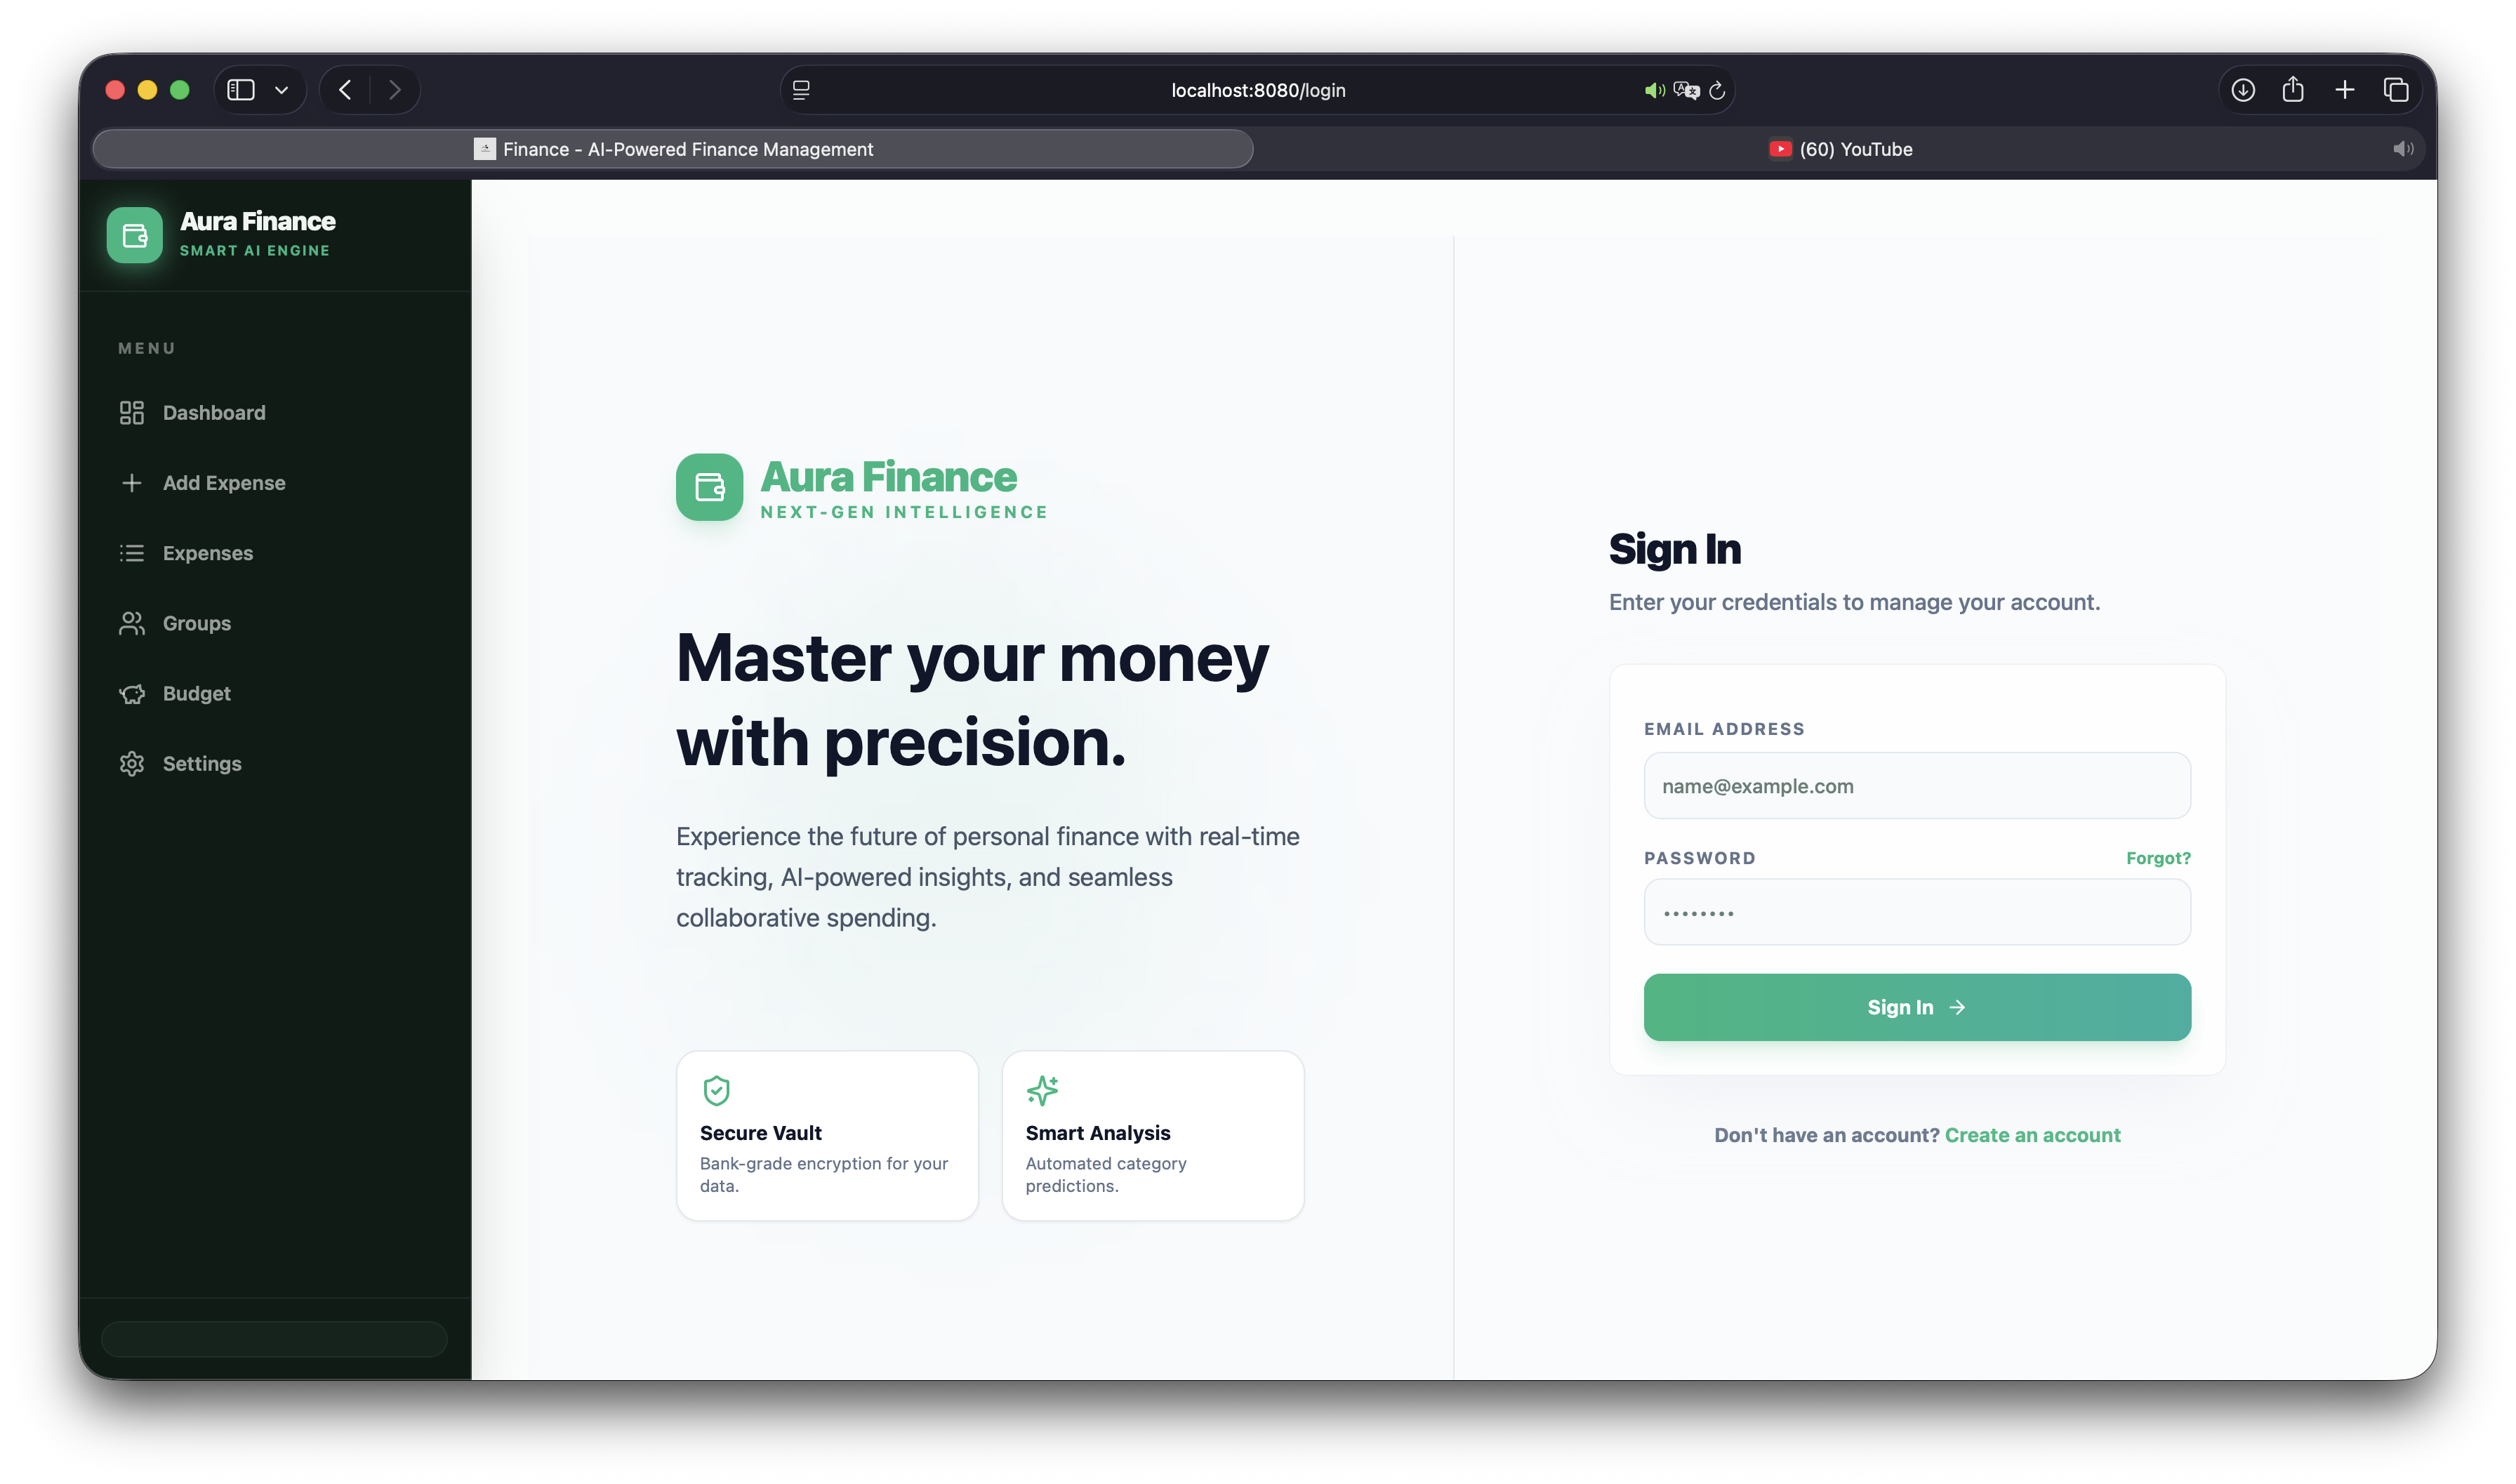
\includegraphics[width=0.8\textwidth]{./fig/aura_sc1} % Placeholder for architecture diagram if available
 \caption{Aura Finance Genel Sistem Mimarisi ve Katmanlı Yapı.}
 \label{fig:mimari_diyagram}
\end{figure}

\section{İstek-Yanıt Döngüsü ve Güvenlik}

Sistemdeki tüm veri trafiği JWT (JSON Web Token) tabanlı kimlik doğrulama ile korunmaktadır. Kullanıcı sisteme giriş yaptığında sunucu tarafından bir token üretilir ve sonraki tüm isteklerde bu token "Authorization" başlığında iletilir. Sunucu, gelen isteği doğrular ve yetki seviyesine göre veritabanı veya AI servislerine erişim sağlar.

\section{Veritabanı Varlık-İlişki Diyagramı (ERD)}

Sistemin kalbinde PostgreSQL veritabanı yer almaktadır. Veri modelleri Prisma ORM kullanılarak yönetilmiştir. Temel tablolar ve ilişkileri aşağıda açıklanmıştır:

\begin{itemize}
    \item \textbf{User (Kullanıcı):} Kimlik bilgileri ve aylık gelir verisi.
    \item \textbf{Expense (Harcama):} Tutar, tarih, kategori ve grup ilişkisi.
    \item \textbf{Budget (Bütçe):} Kategori bazlı limitler.
    \item \textbf{Category (Kategori):} Sabit harcama kategorileri (Gıda, Ulaşım, vb.).
\end{itemize}

Şekil~\ref{fig:erd_diyagram} veritabanı şemasını ve tablolar arası ilişkileri temsil etmektedir.

\begin{figure}[h!]
 \centering
 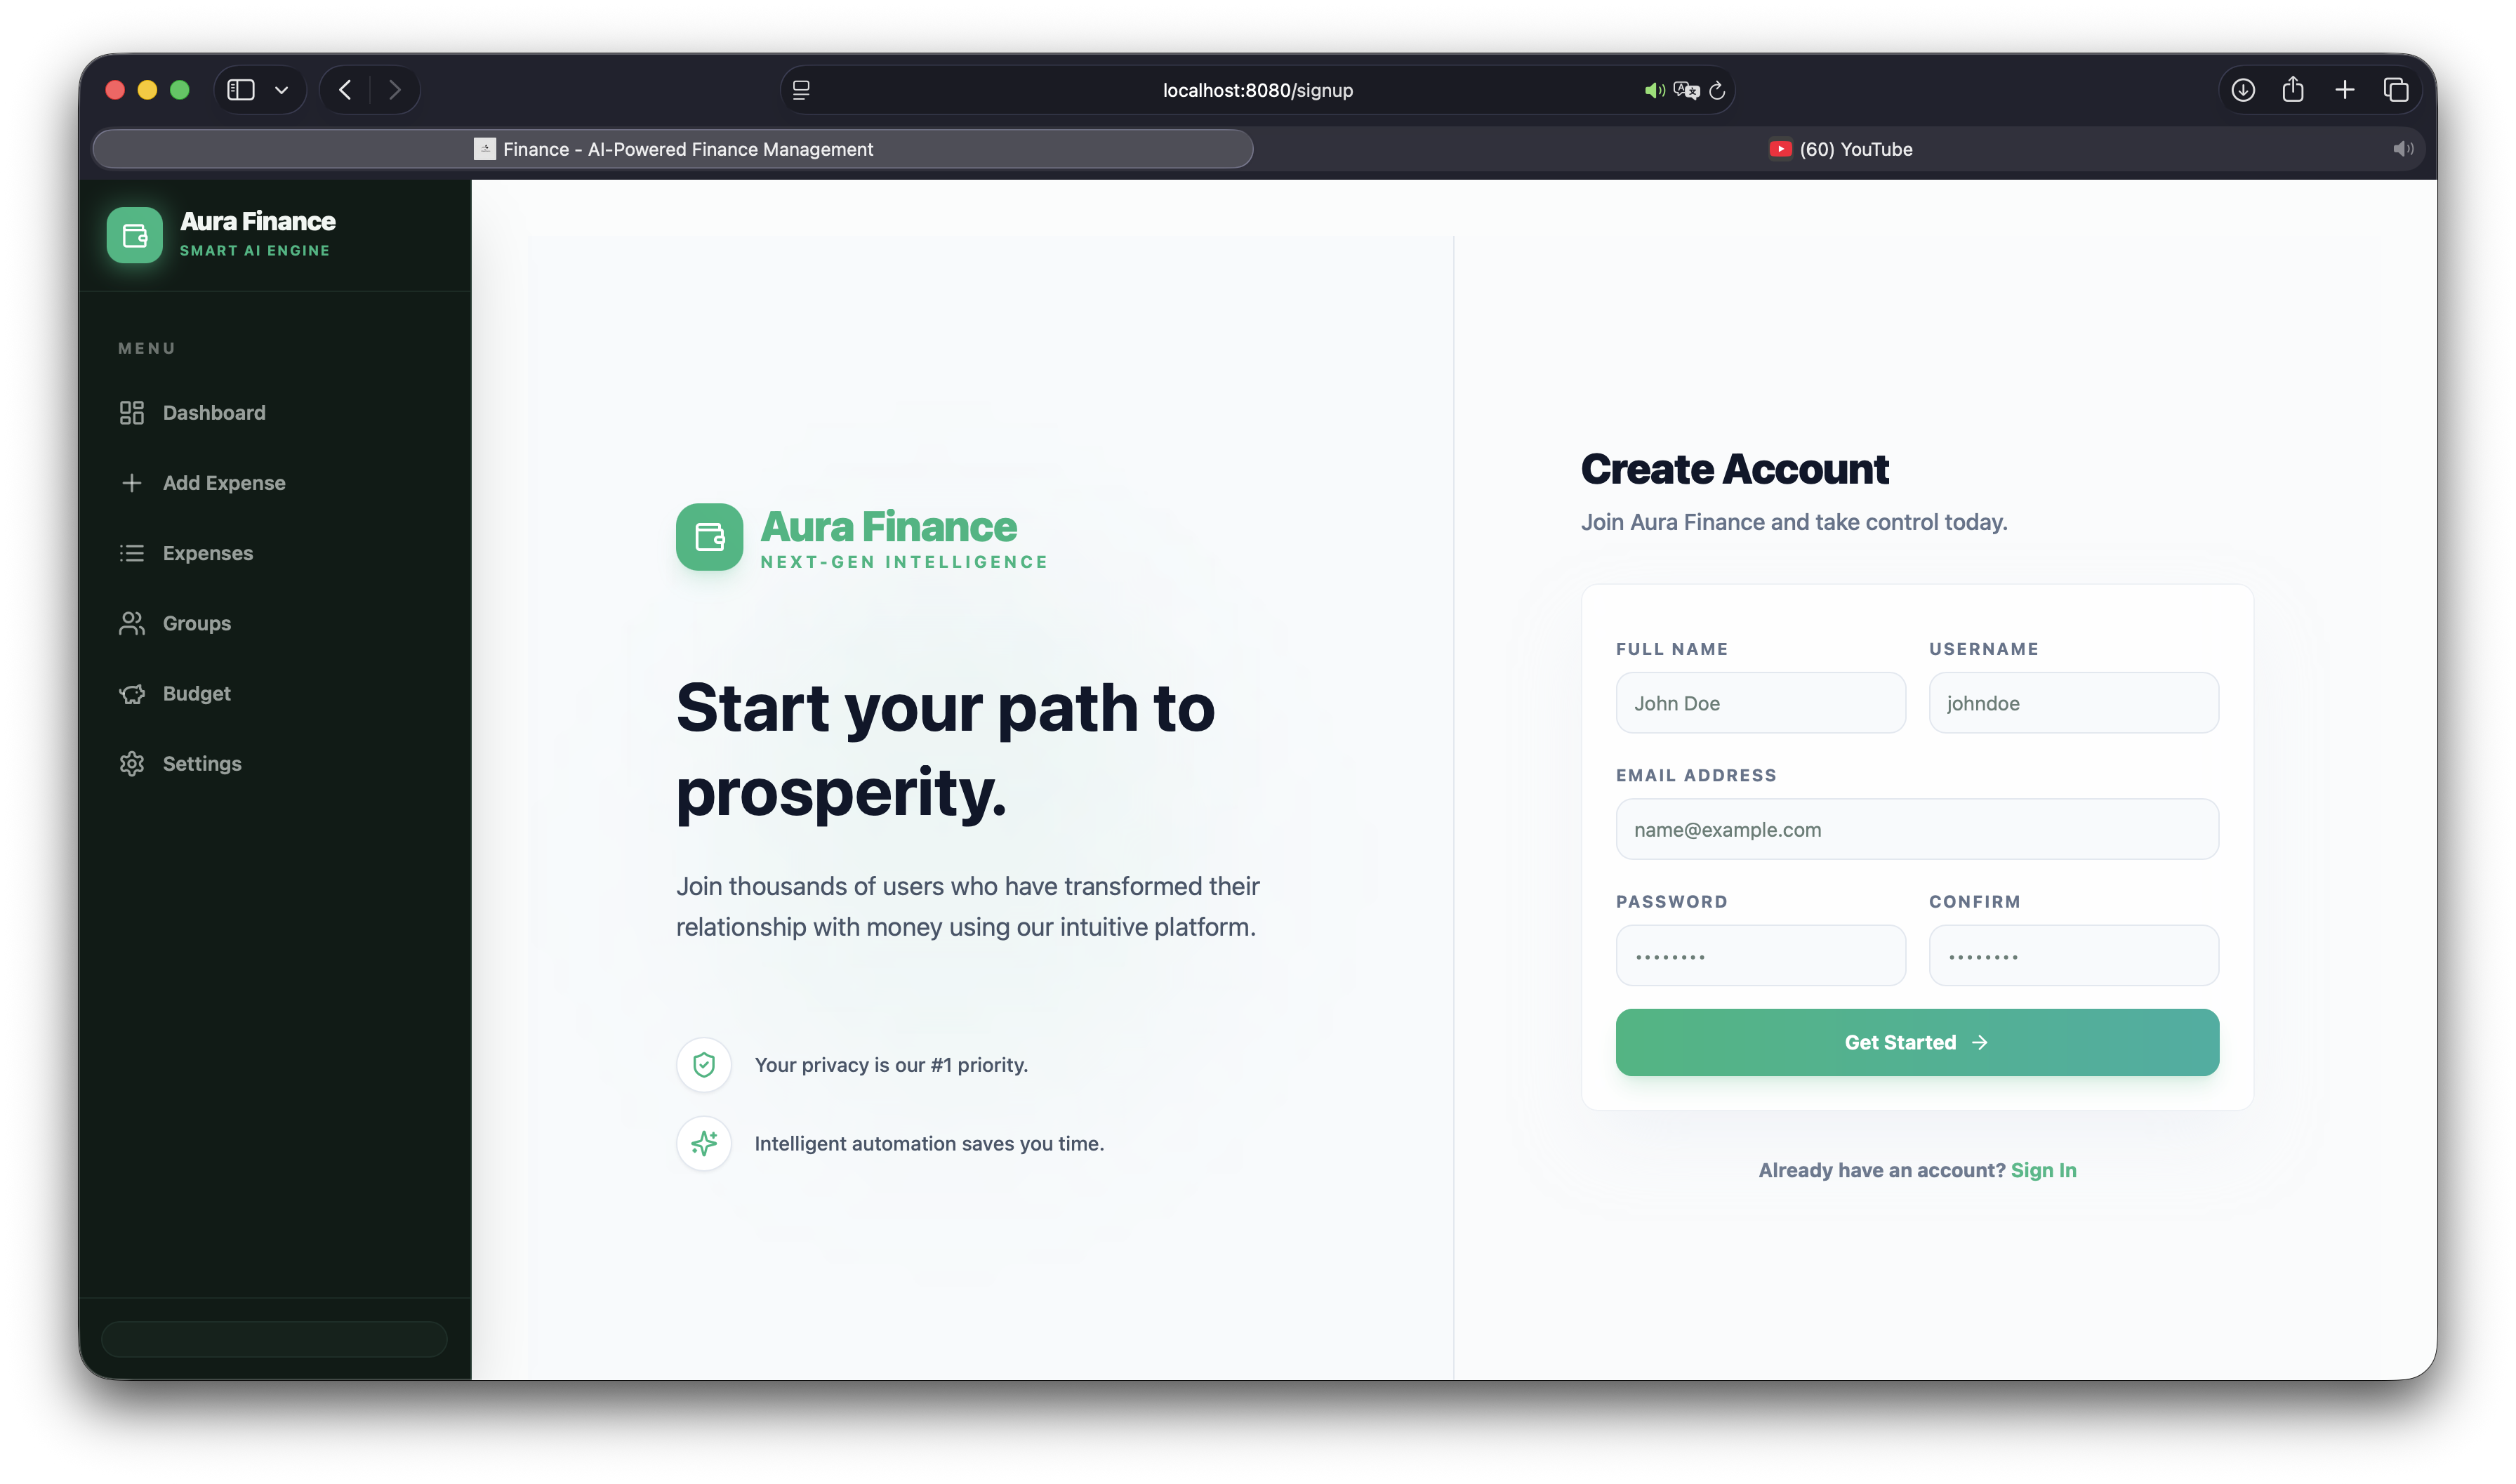
\includegraphics[width=0.7\textwidth]{./fig/aura_sc2} % Placeholder for ERD
 \caption{Veritabanı Varlık-İlişki Diyagramı (ERD).}
 \label{fig:erd_diyagram}
\end{figure}

\section{Teknoloji Yığını}

Aura Finance, yüksek performans ve tip güvenliği için \textbf{TypeScript} ile yazılmış bir \textbf{React} uygulamasıdır. Sunucu tarafında \textbf{Node.js} ve \textbf{Express.js} kullanılmış, veritabanı işlemleri için \textbf{Prisma} tercih edilmiştir. Yapay zekâ modülleri ise \textbf{TensorFlow.js} ve \textbf{XGBoost} ile hibrit bir yapıda kurgulanmıştır.

\clearpage

\chapter{TEKNİK UYGULAMA}

Bu bölümde Aura Finance uygulamasının temel işlevlerinin teknik gerçekleştirimi ve algoritma detayları sunulmaktadır.

\section{Kullanıcı Kimlik Doğrulama ve Güvenlik}

Uygulama, güvenli bir oturum yönetimi için JSON Web Token (JWT) tabanlı stateless (durum bilgisi saklamayan) bir yapı kullanır.
\begin{itemize}
    \item \textbf{Kayıt Olma:} Kullanıcı şifreleri sunucuya ulaştığında \texttt{bcryptjs} kütüphanesi kullanılarak tuzlanmış (salted) bir şekilde karma (hash) işlemine tabi tutulur.
    \item \textbf{Giriş Yapma:} Başarılı giriş sonrası sunucu, kullanıcının kimlik bilgilerini içeren ve 7 gün geçerliliği olan bir JWT imzalar.
    \item \textbf{Yetkilendirme:} İstemci tarafındaki her hassas istek (harcama ekleme, bütçe görüntüleme vb.), HTTP "Authorization" başlığında bu token'ı taşır.
\end{itemize}

\section{Harcama Yönetimi ve Veri İşleme}

Harcama yönetimi modülü, kullanıcılara esnek bir veri giriş imkanı sunar. Harcamalar PostgreSQL üzerinde \texttt{Expense} tablosunda saklanır. React tarafında \texttt{useExpenses} hook'u, \texttt{React Query} kullanarak verilerin önbelleğe alınmasını ve sunucu ile asenkron senkronizasyonunu yönetir.

\section{Akıllı Veri Giriş Yöntemleri}

Uygulamanın en önemli özelliklerinden biri, veri girişini kolaylaştıran yardımcı teknolojilerdir.

\subsection{OCR ile Makbuz Okuma}
İstemci tarafında çalışan \texttt{Tesseract.js} motoru sayesinde kullanıcılar makbuz fotoğraflarını yükleyebilirler. Uygulama, görüntüden çıkarılan metin içindeki anahtar kelimeleri (örneğin: "Toplam", "Market", "Benzin") analiz ederek harcama miktarını ve kategorisini otomatik olarak tahmin eder.

\subsection{Sesli Komut ile Harcama Ekleme}
Web Speech API kullanılarak gerçekleştirilen bu özellikte, kullanıcının sesli ifadesi (örneğin: "Yemek için 250 lira harcadım") metne dönüştürülür. Sunucu tarafındaki bir düzenli ifade (regex) analizörü, bu metinden sayısal miktarı ve kategori ismini ayıklayarak formu otomatik doldurur.

\section{AI Insights (Yapay Zekâ İçgörüleri)}

Sunucu tarafında çalışan bir analiz motoru, kullanıcının geçmiş harcama verilerini tarayarak aşağıdaki içgörüleri üretir:
\begin{itemize}
    \item \textbf{Abonelik Tespiti:} Belirli aralıklarla tekrarlanan aynı miktardaki harcamaları tespit eder.
    \item \textbf{Anomali Tespiti:} Kullanıcının alışılagelmiş harcama ortalamasının 2.5 katı üzerindeki işlemleri "Olağandışı Harcama" olarak işaretler.
    \item \textbf{Hız Analizi:} Ayın mevcut günündeki harcama hızını kullanarak ay sonu toplam harcama tahmininde bulunur.
\end{itemize}

\clearpage

\chapter{YAPAY ZEKÂ VE METODOLOJİ}

Aura Finance, kullanıcıların finansal kararlarını desteklemek için iki temel yapay zekâ yaklaşımı kullanmaktadır: Zaman serisi tahmini (LSTM) ve bütçe optimizasyonu (XGBoost).

\section{Harcama Tahmini: LSTM Modeli}

Kullanıcıların gelecek ay ne kadar harcama yapacağını tahmin etmek için Uzun Kısa Süreli Bellek (Long Short-Term Memory - LSTM) ağları kullanılmıştır. Bu model, Node.js üzerinde \texttt{TensorFlow.js} kütüphanesi ile gerçek zamanlı olarak çalıştırılmaktadır.

\subsection{Model Mimarisi}
Model, ardışık (sequential) bir yapıdadır ve şu katmanlardan oluşur: LSTM katmanı (32 birim, \%10 dropout), Yoğun katman (16 birim, ReLU) ve Çıkış katmanı (1 birim, sigmoid).

\subsection{Eğitim Süreci}
Model, kullanıcının geçmiş harcama verilerini pencereleme (windowing) yöntemiyle işler. Veriler eğitim öncesinde [0, 1] aralığına normalleştirilir. Adam optimizasyon algoritması kullanılarak eğitilir.

\section{Bütçe Optimizasyonu: XGBoost Regresyonu}

Kullanıcıların gelirlerine göre ideal bütçe dağılımını belirlemek için Python tabanlı bir makine öğrenmesi modeli geliştirilmiştir. Eğitim için \texttt{Indian\_Finance\_Dataset.csv} kullanılmıştır. Model olarak \texttt{MultiOutputRegressor} mimarisiyle XGBoost algoritması tercih edilmiştir.

\section{Hibrit Dürtme (Nudge) Algoritması}

Sistemin en özgün yanlarından biri, statik bütçe önerileri yerine kullanıcının mevcut alışkanlıklarını da hesaba katan hibrit bir mantık yürütmesidir. İdeal bütçe ($B_{ideal}$) ve kullanıcının gerçek harcama ortalaması ($B_{gercek}$) arasındaki denge şu formülle hesaplanır:

\begin{equation}
   B_{oneri} = (B_{ideal} \times 0.70) + (B_{gercek} \times 0.30)
\end{equation}

Bu yaklaşım, kullanıcıyı ideal finansal hedeflere yönlendirirken, mevcut yaşam standartlarını da göz ardı etmeyerek gerçekçi bütçe hedefleri sunar.

\clearpage

\chapter{UYGULAMA VE BULGULAR}

Aura Finance uygulaması, geliştirilen mimari ve algoritmaların birleşimiyle tam fonksiyonel bir finansal yönetim platformu olarak hayata geçirilmiştir. Bu bölümde, uygulamanın kullanıcı arayüzü ve elde edilen bulgular ekran görüntüleri eşliğinde sunulmaktadır.

\section{Kullanıcı Arayüzü Analizi}

Uygulamanın arayüzü, kullanıcı deneyimini (UX) ön planda tutan modern ve responsive bir yapıdadır.

\begin{figure}[h!]
 \centering
 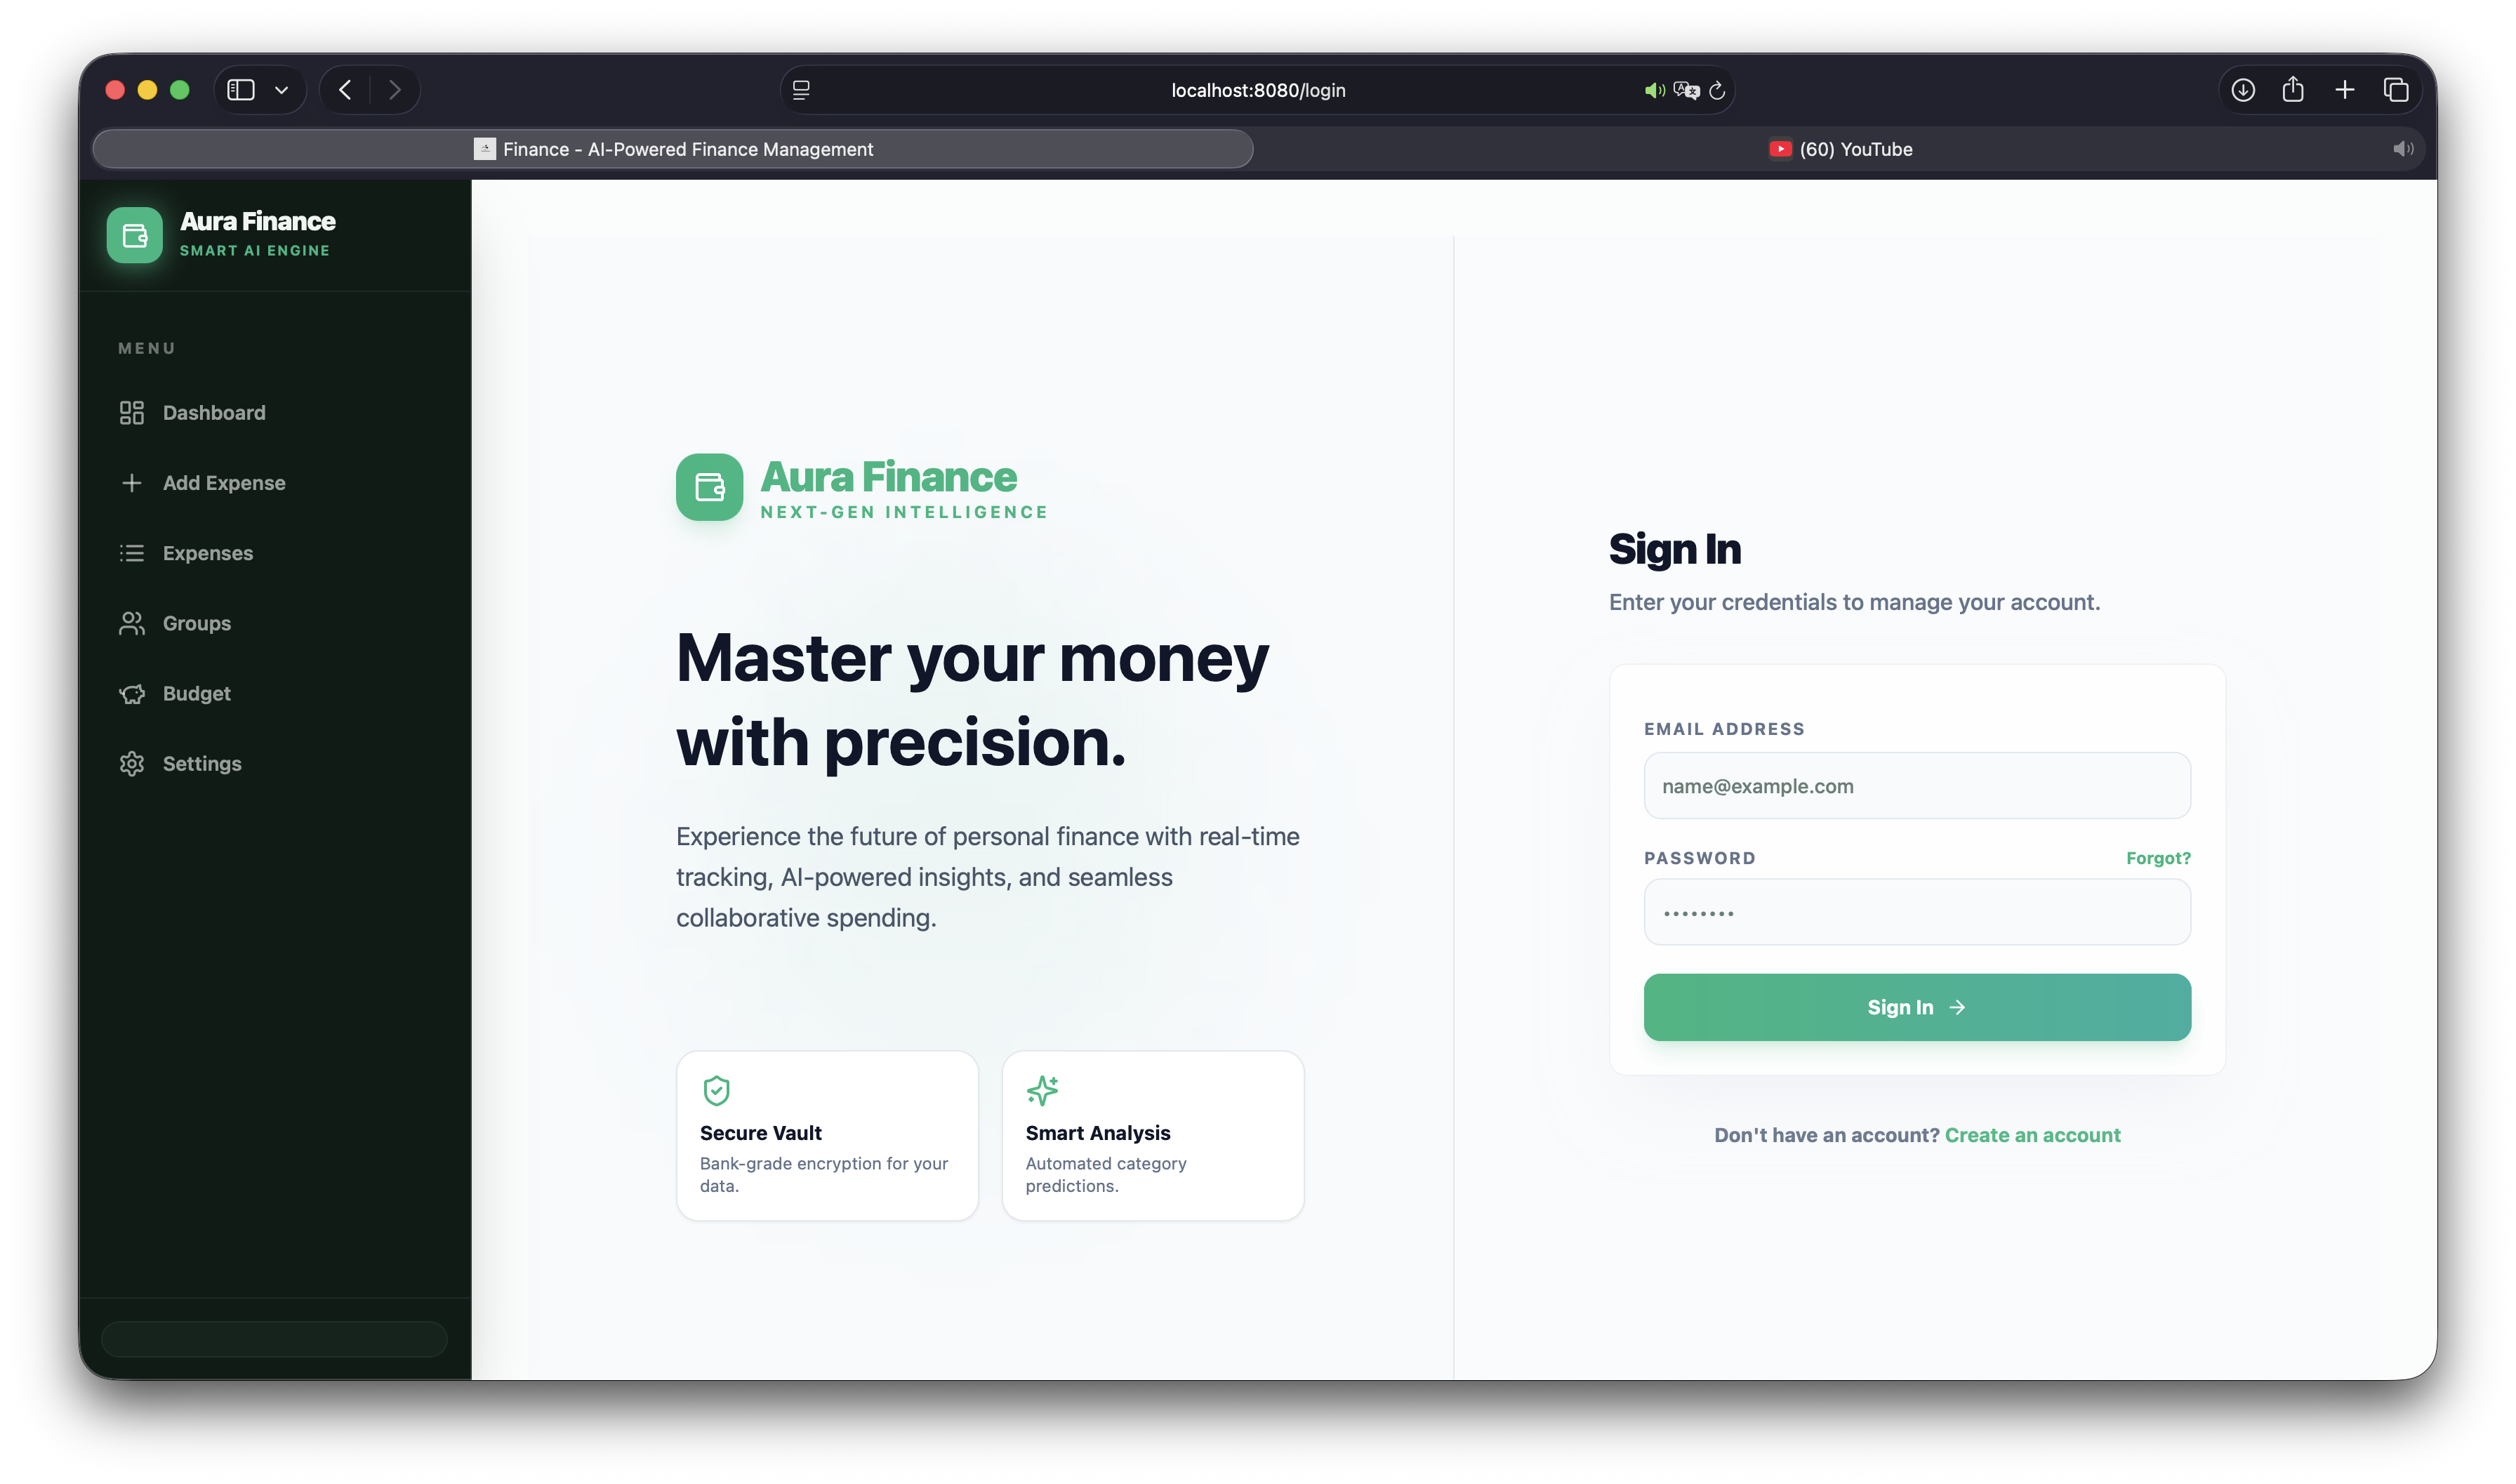
\includegraphics[width=0.8\textwidth]{./fig/aura_sc1}
 \caption{Aura Finance Ana Gösterge Paneli (Dashboard).}
 \label{fig:sc1}
\end{figure}

\begin{figure}[h!]
 \centering
 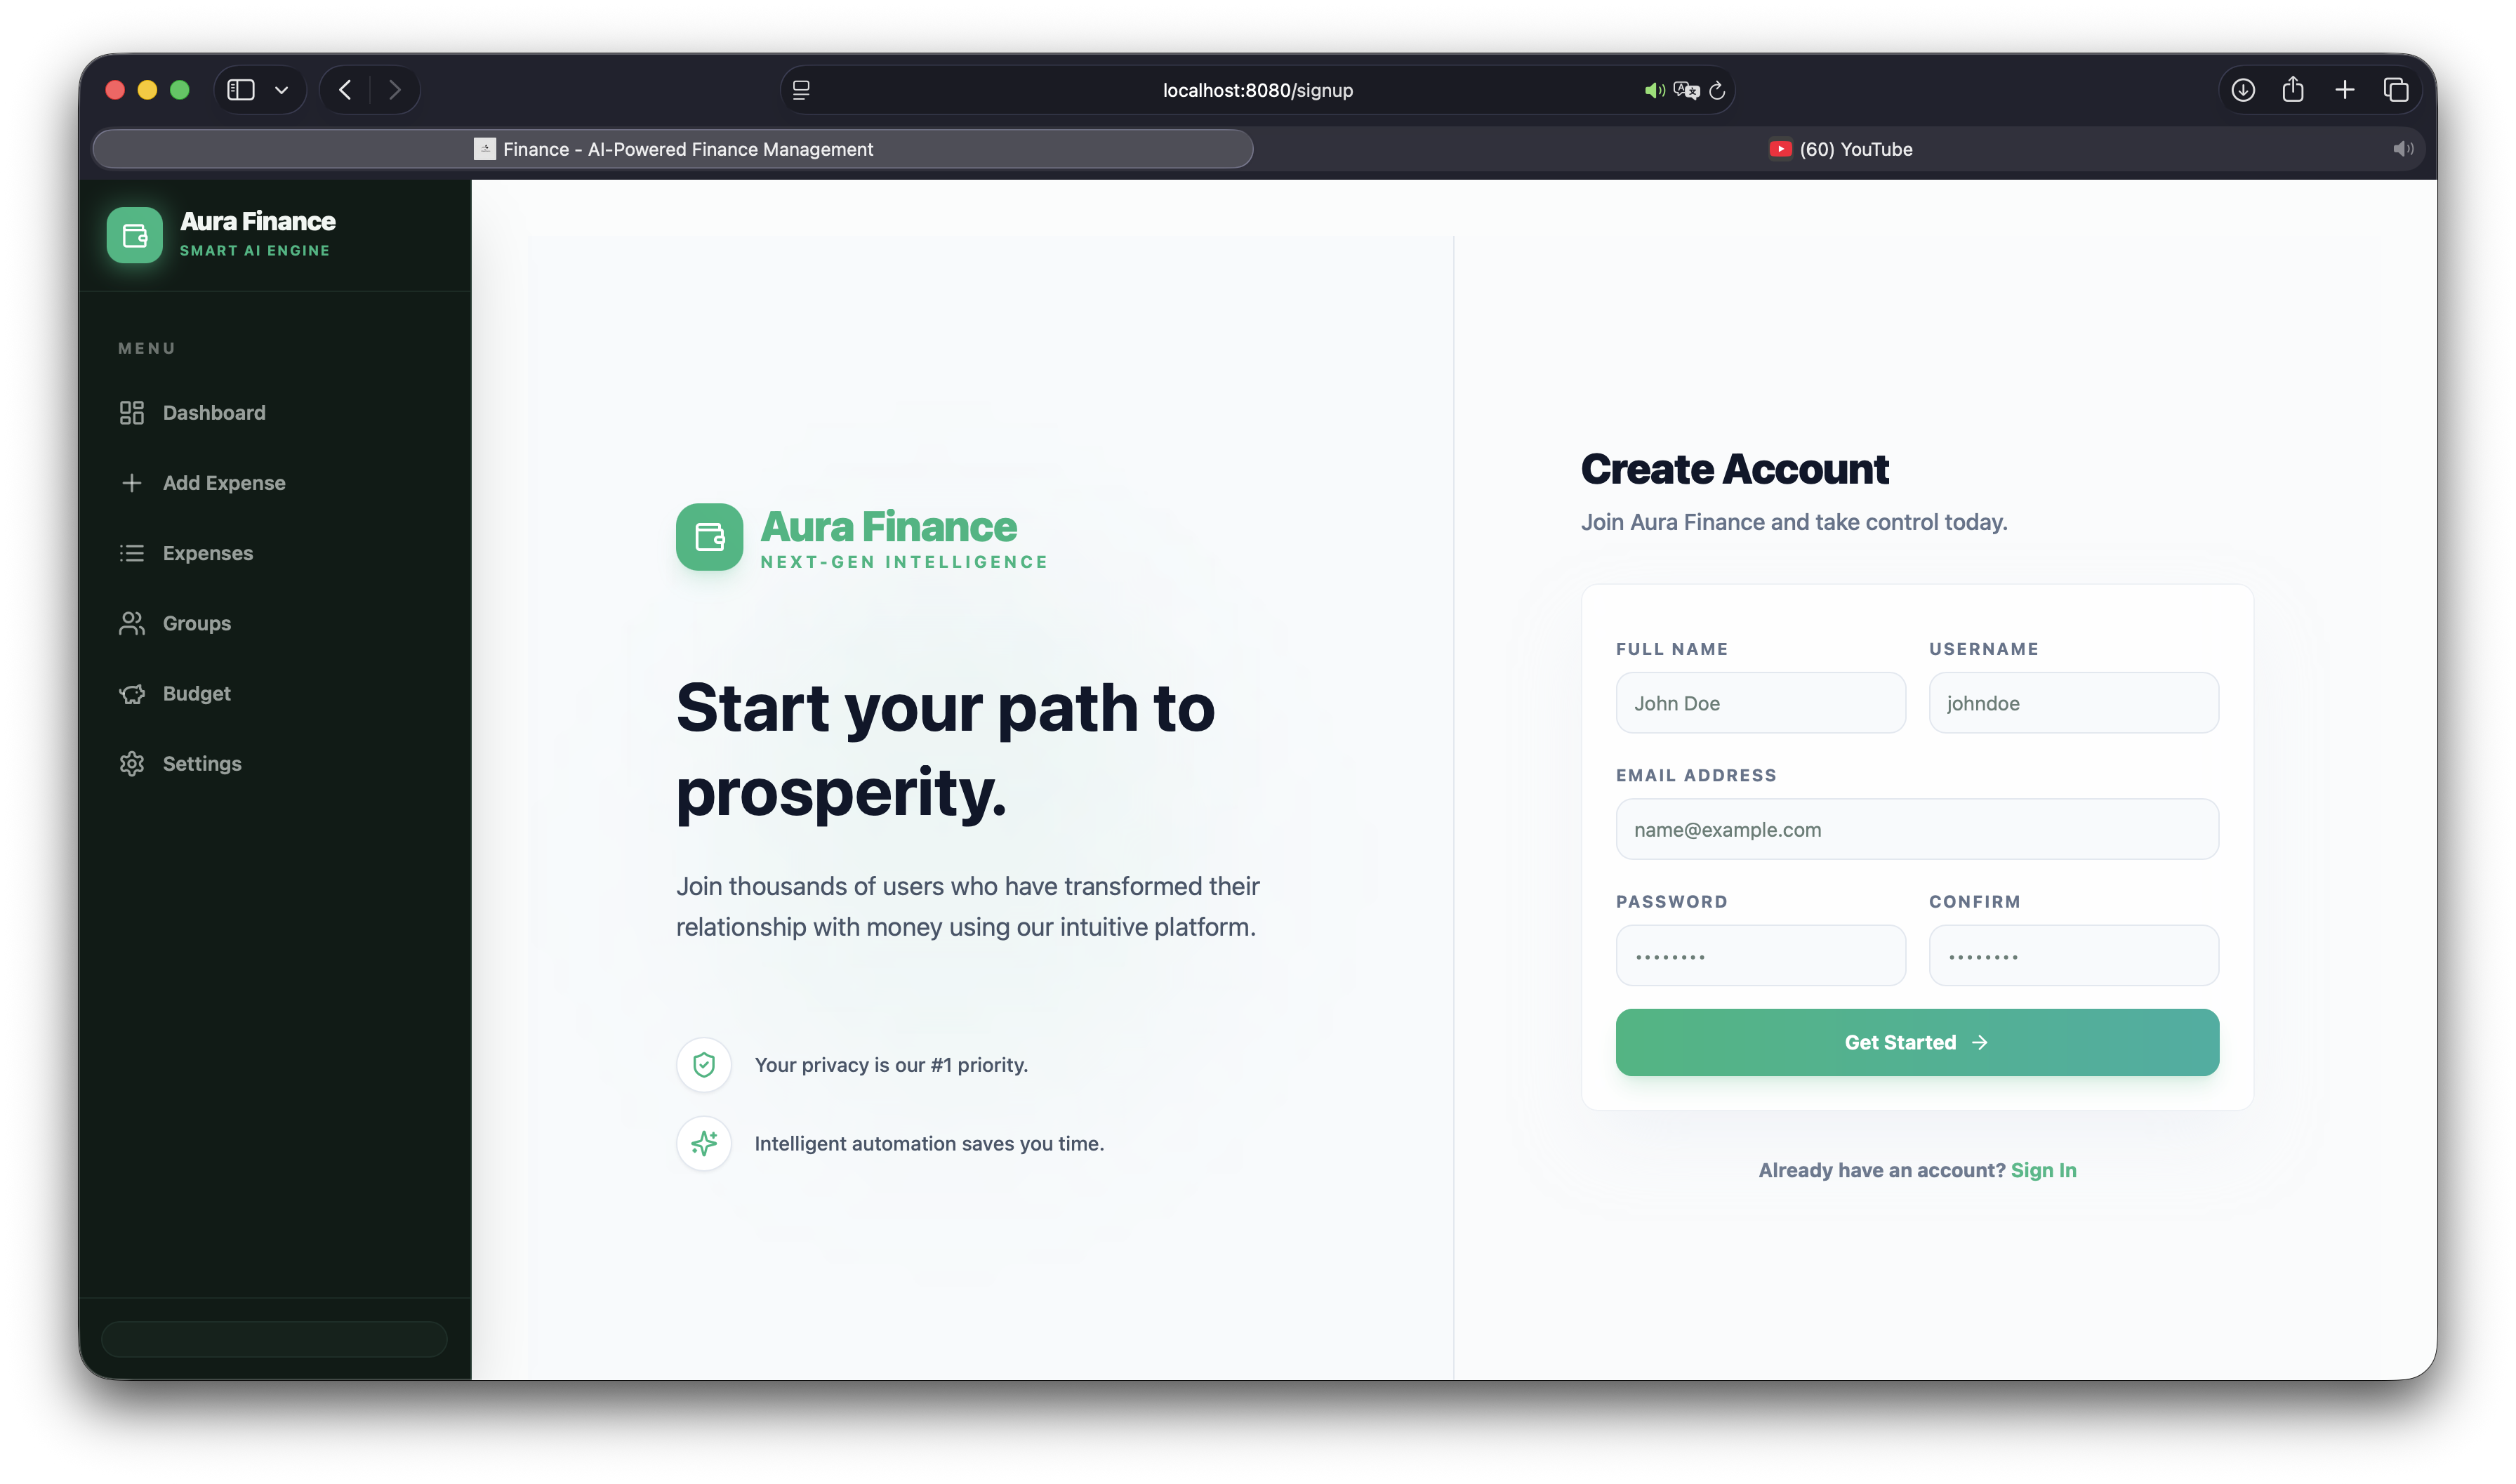
\includegraphics[width=0.8\textwidth]{./fig/aura_sc2}
 \caption{Kullanıcı Harcama Geçmişi ve Analitiği.}
 \label{fig:sc2}
\end{figure}

\begin{figure}[h!]
 \centering
 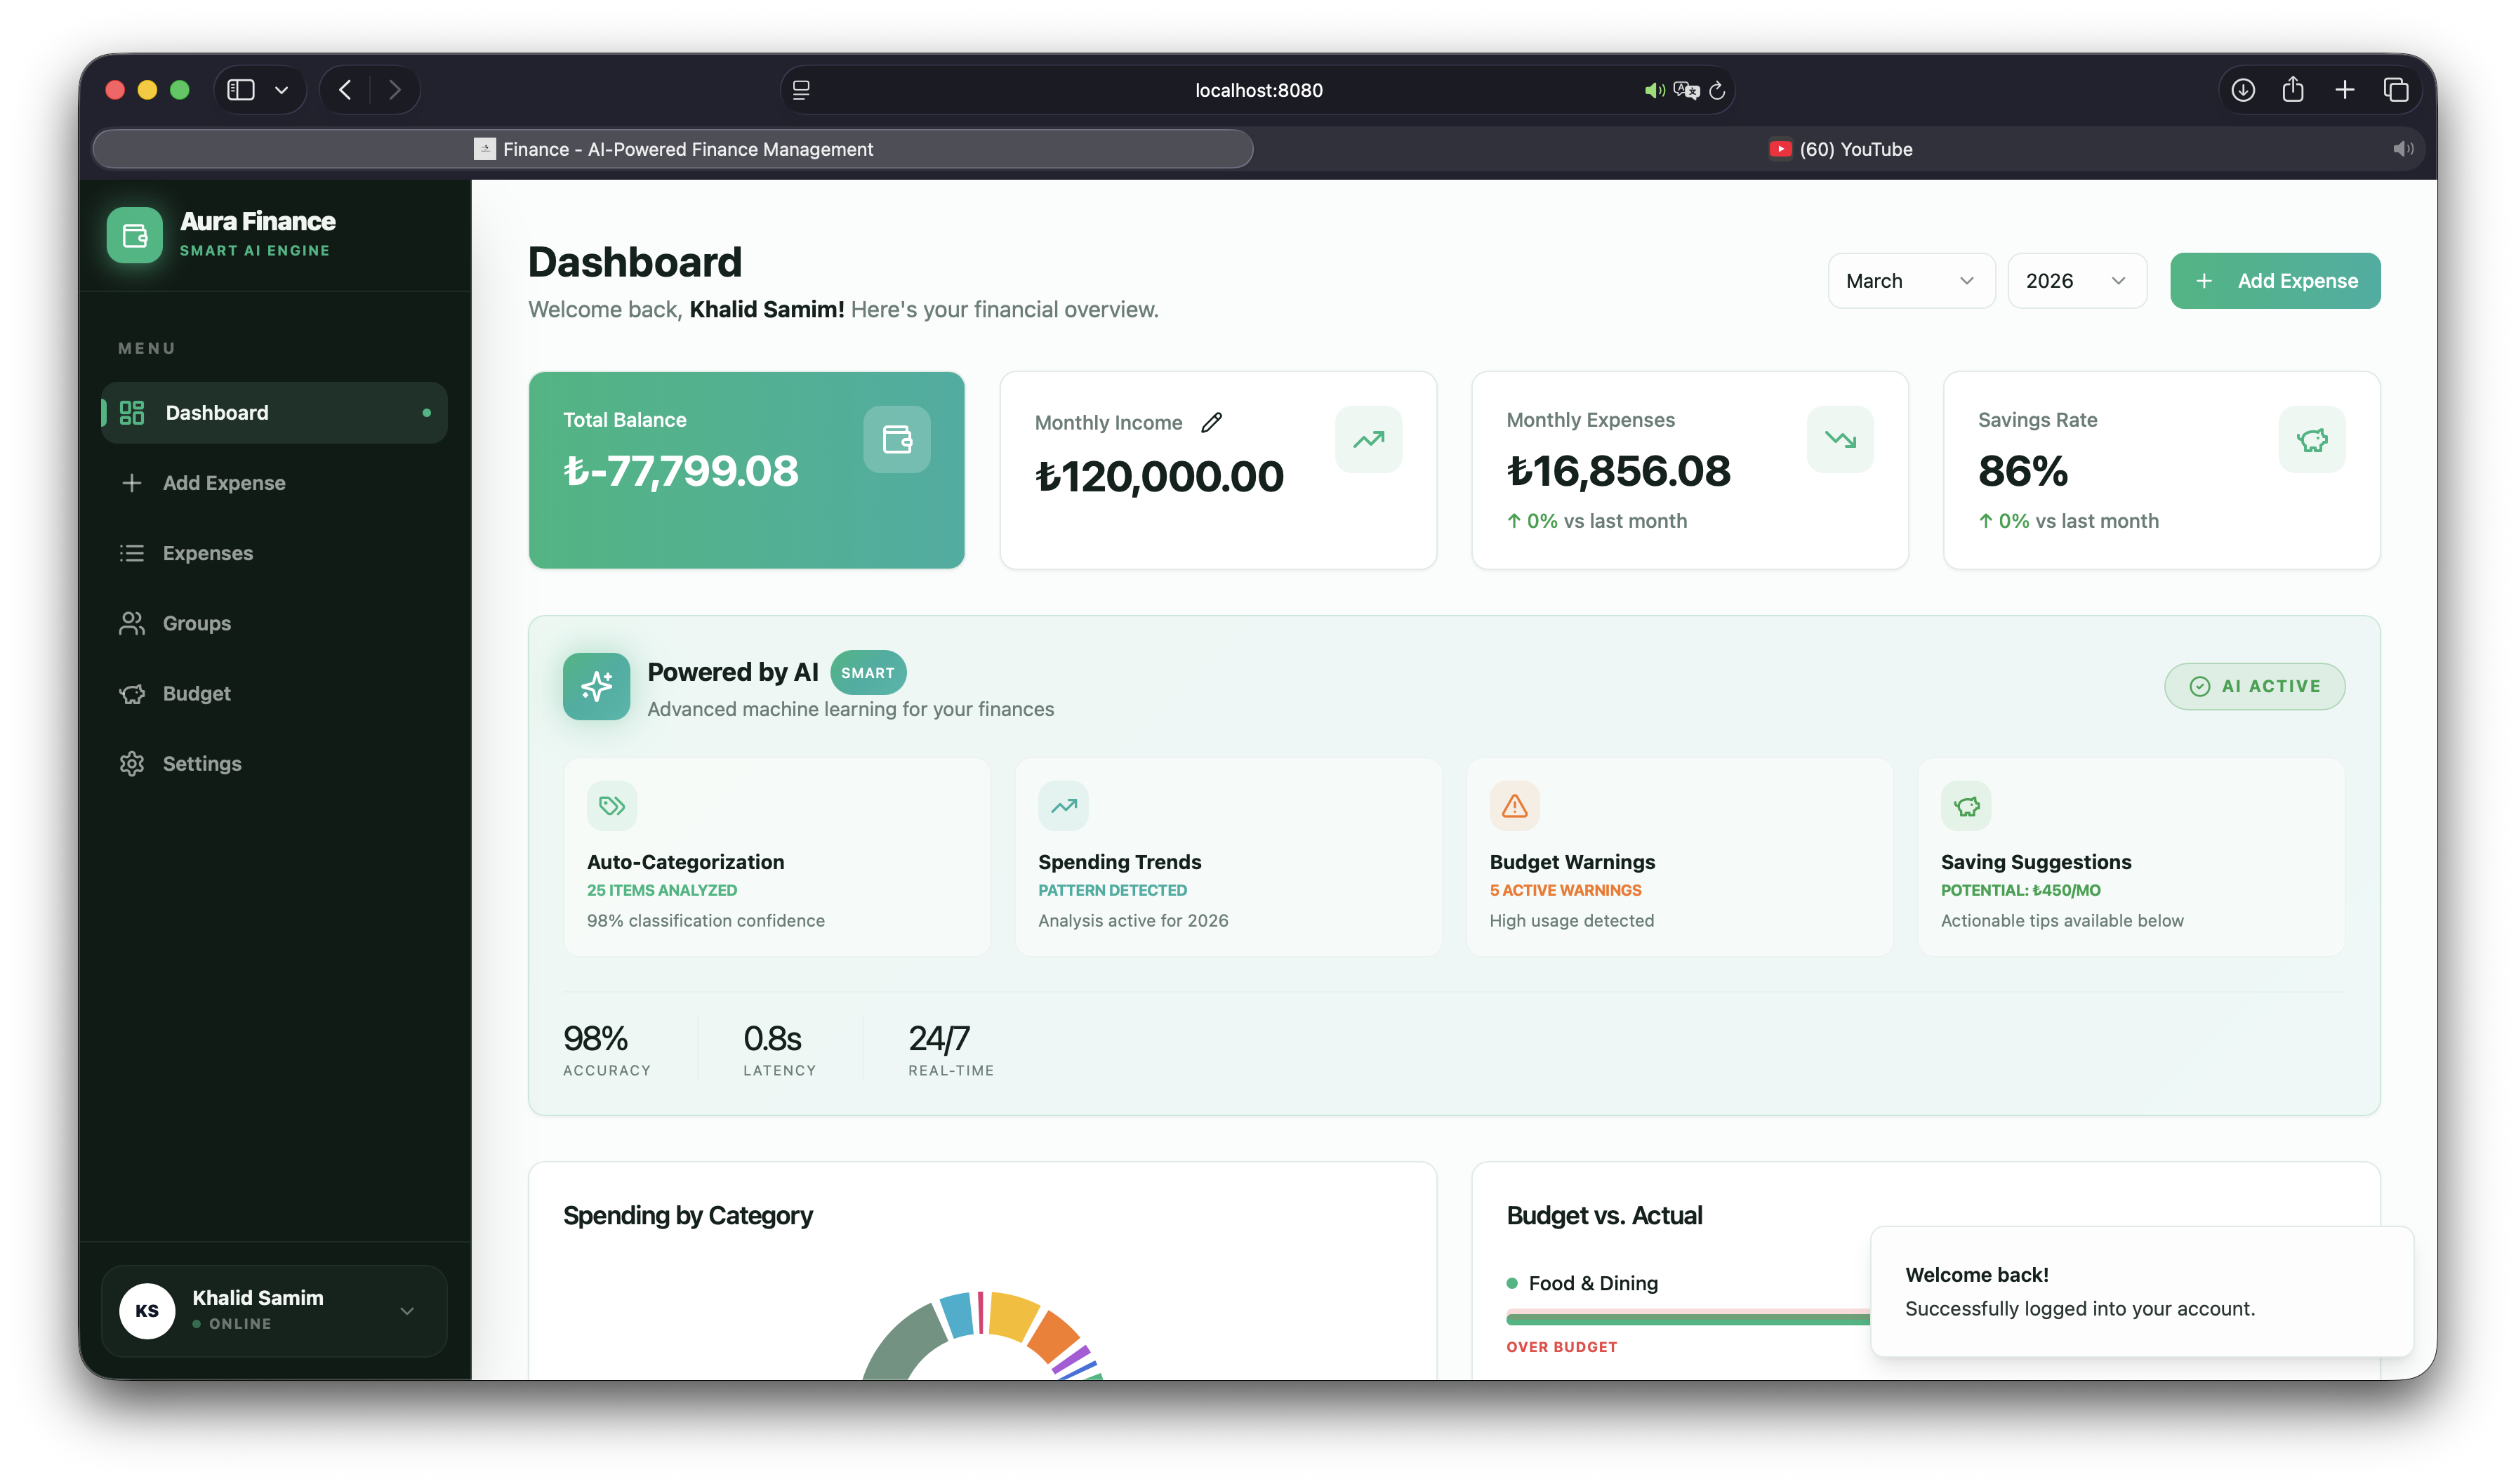
\includegraphics[width=0.8\textwidth]{./fig/aura_sc3}
 \caption{Harcama Filtreleme ve Kategori Bazlı Listeleme.}
 \label{fig:sc3}
\end{figure}

\section{Yapay Zekâ ve Tahminleme Bulguları}

Uygulamanın yapay zekâ modülleri, kullanıcıların finansal sağlığını korumak adına proaktif çözümler sunmaktadır.

\begin{figure}[h!]
 \centering
 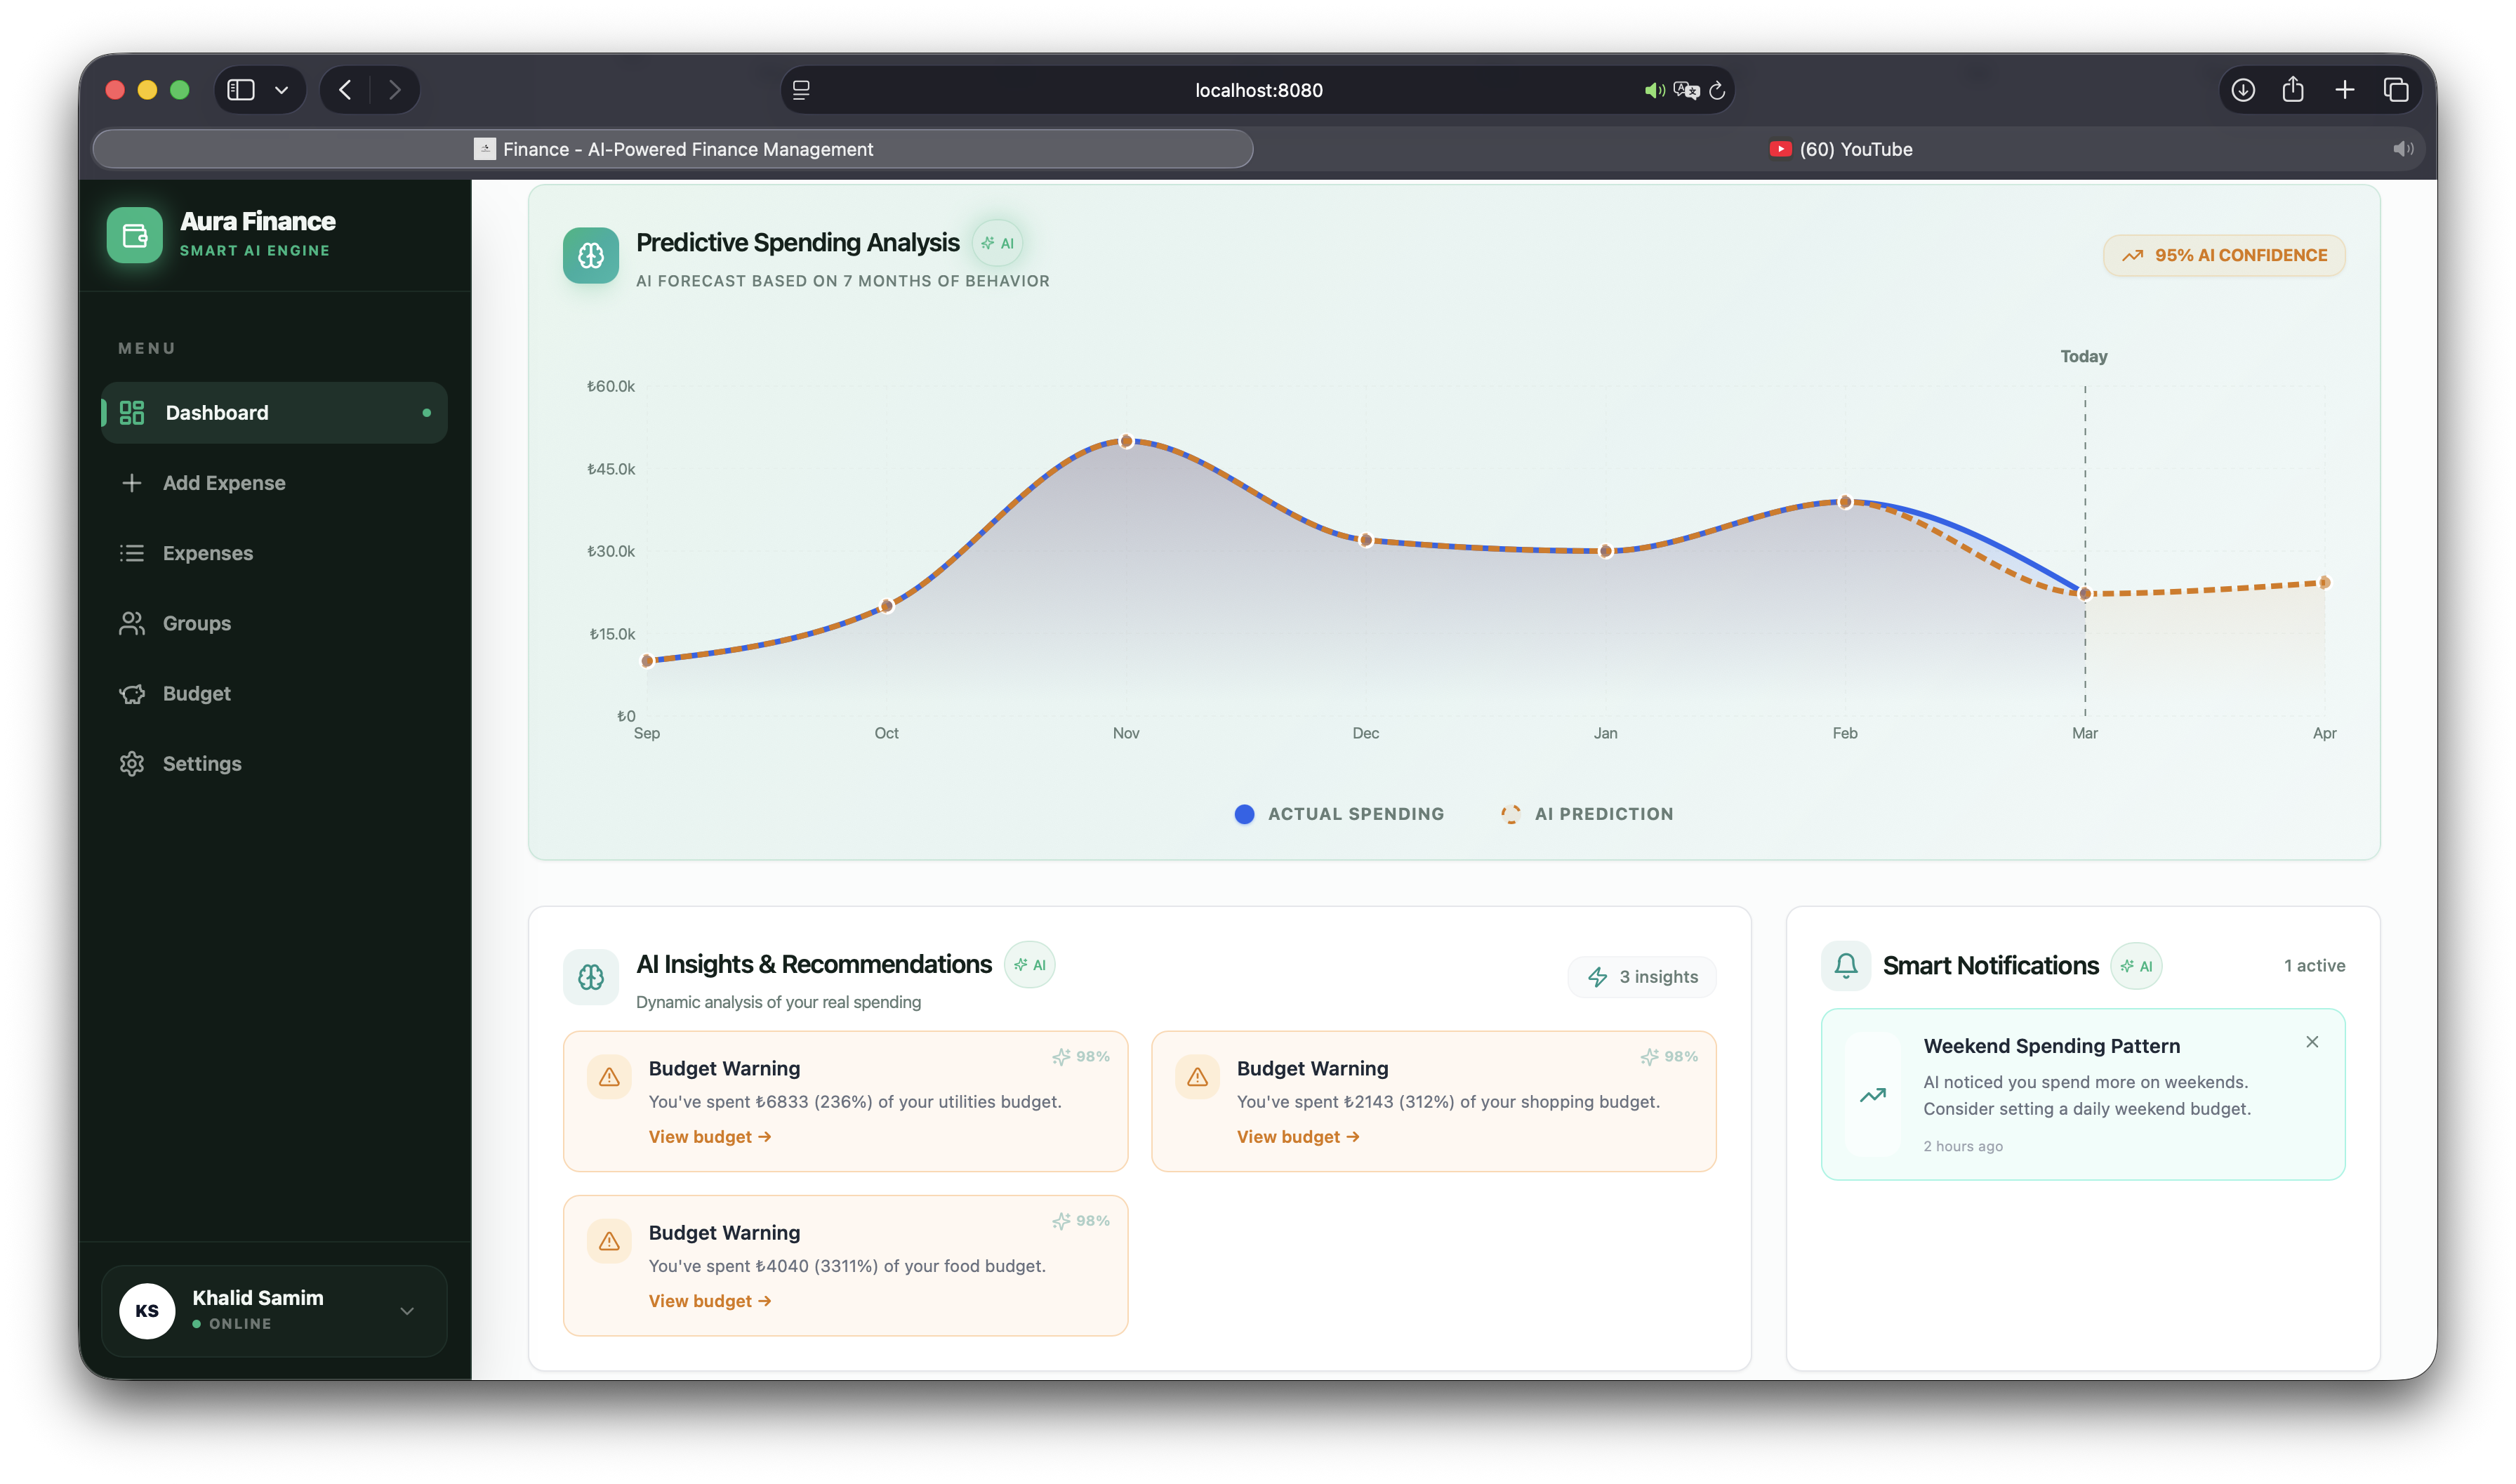
\includegraphics[width=0.8\textwidth]{./fig/aura_sc4}
 \caption{AI Insights: Otomatik Harcama Analizi ve Bildirimler.}
 \label{fig:sc4}
\end{figure}

\begin{figure}[h!]
 \centering
 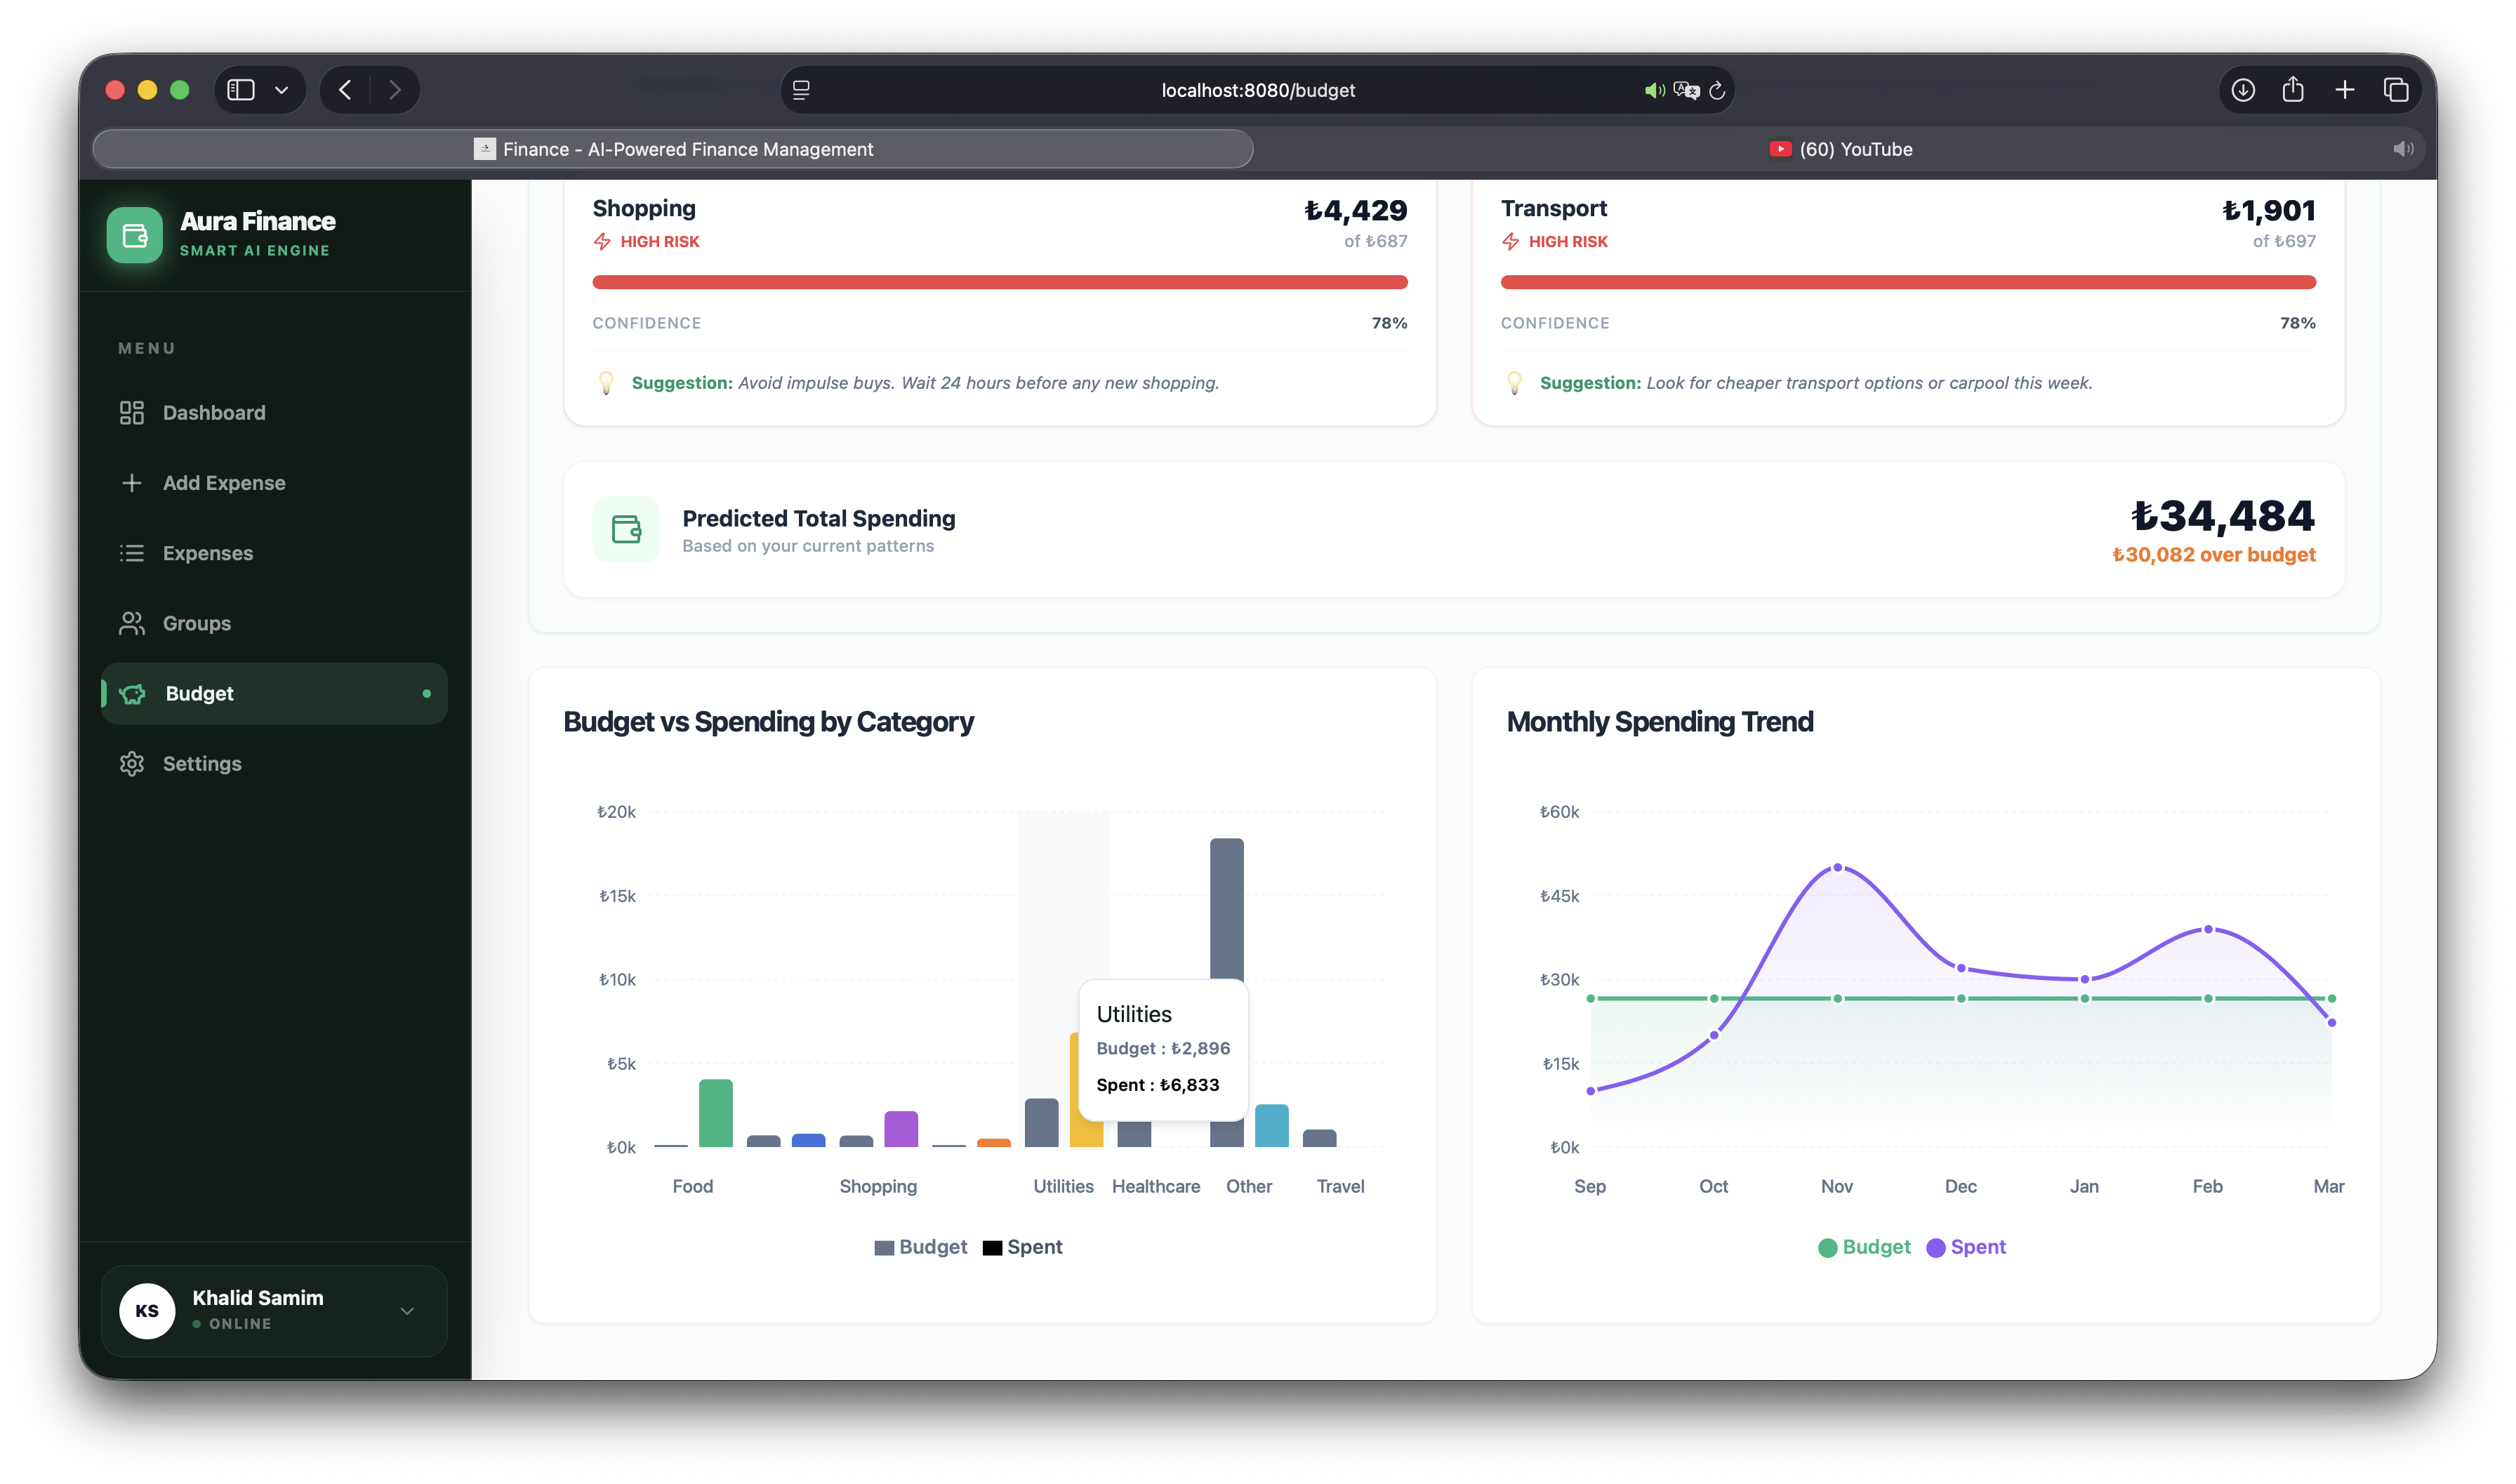
\includegraphics[width=0.8\textwidth]{./fig/aura_sc9}
 \caption{Hibrit Bütçe Optimizasyon Önerileri.}
 \label{fig:sc9}
\end{figure}

\begin{figure}[h!]
 \centering
 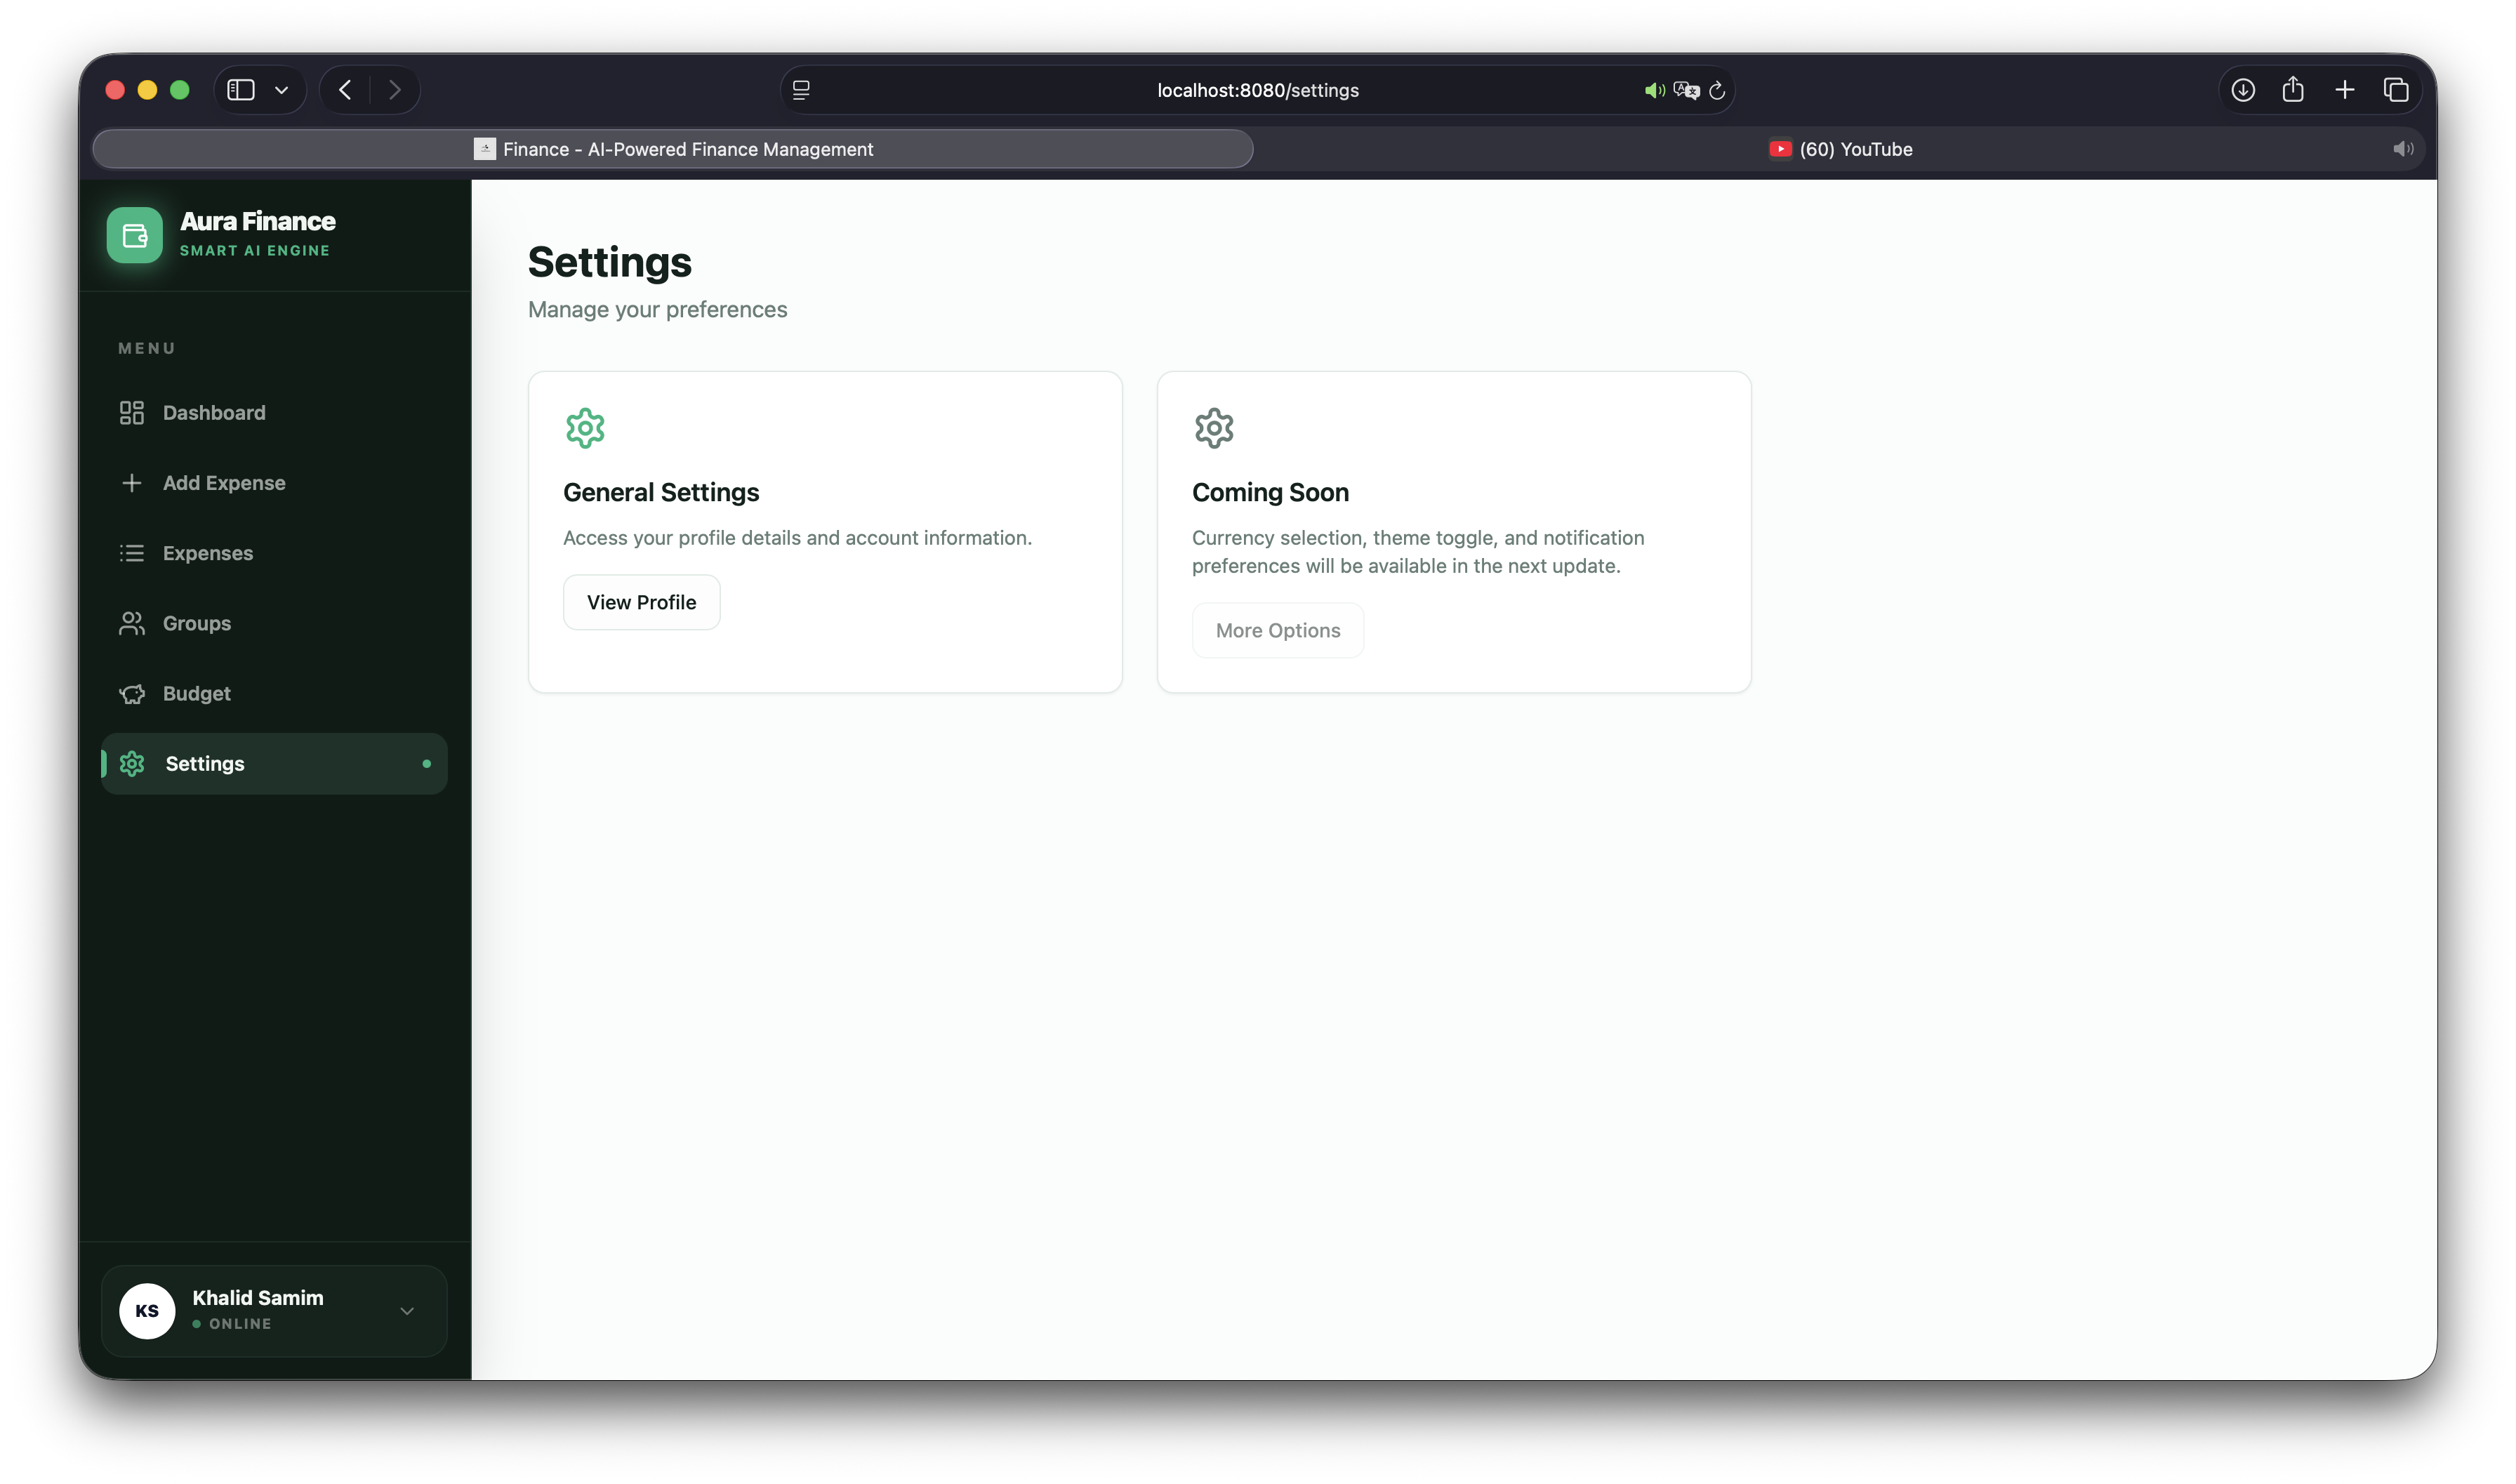
\includegraphics[width=0.8\textwidth]{./fig/aura_sc10}
 \caption{LSTM Tabanlı Gelecek Ay Harcama Tahmin Grafiği.}
 \label{fig:sc10}
\end{figure}

\section{Akıllı Veri Giriş Yöntemleri ve Gruplar}

OCR ve sesli komut teknolojileri, veri giriş sürecini otomatize ederek kullanıcı yükünü azaltmaktadır.

\begin{figure}[h!]
 \centering
 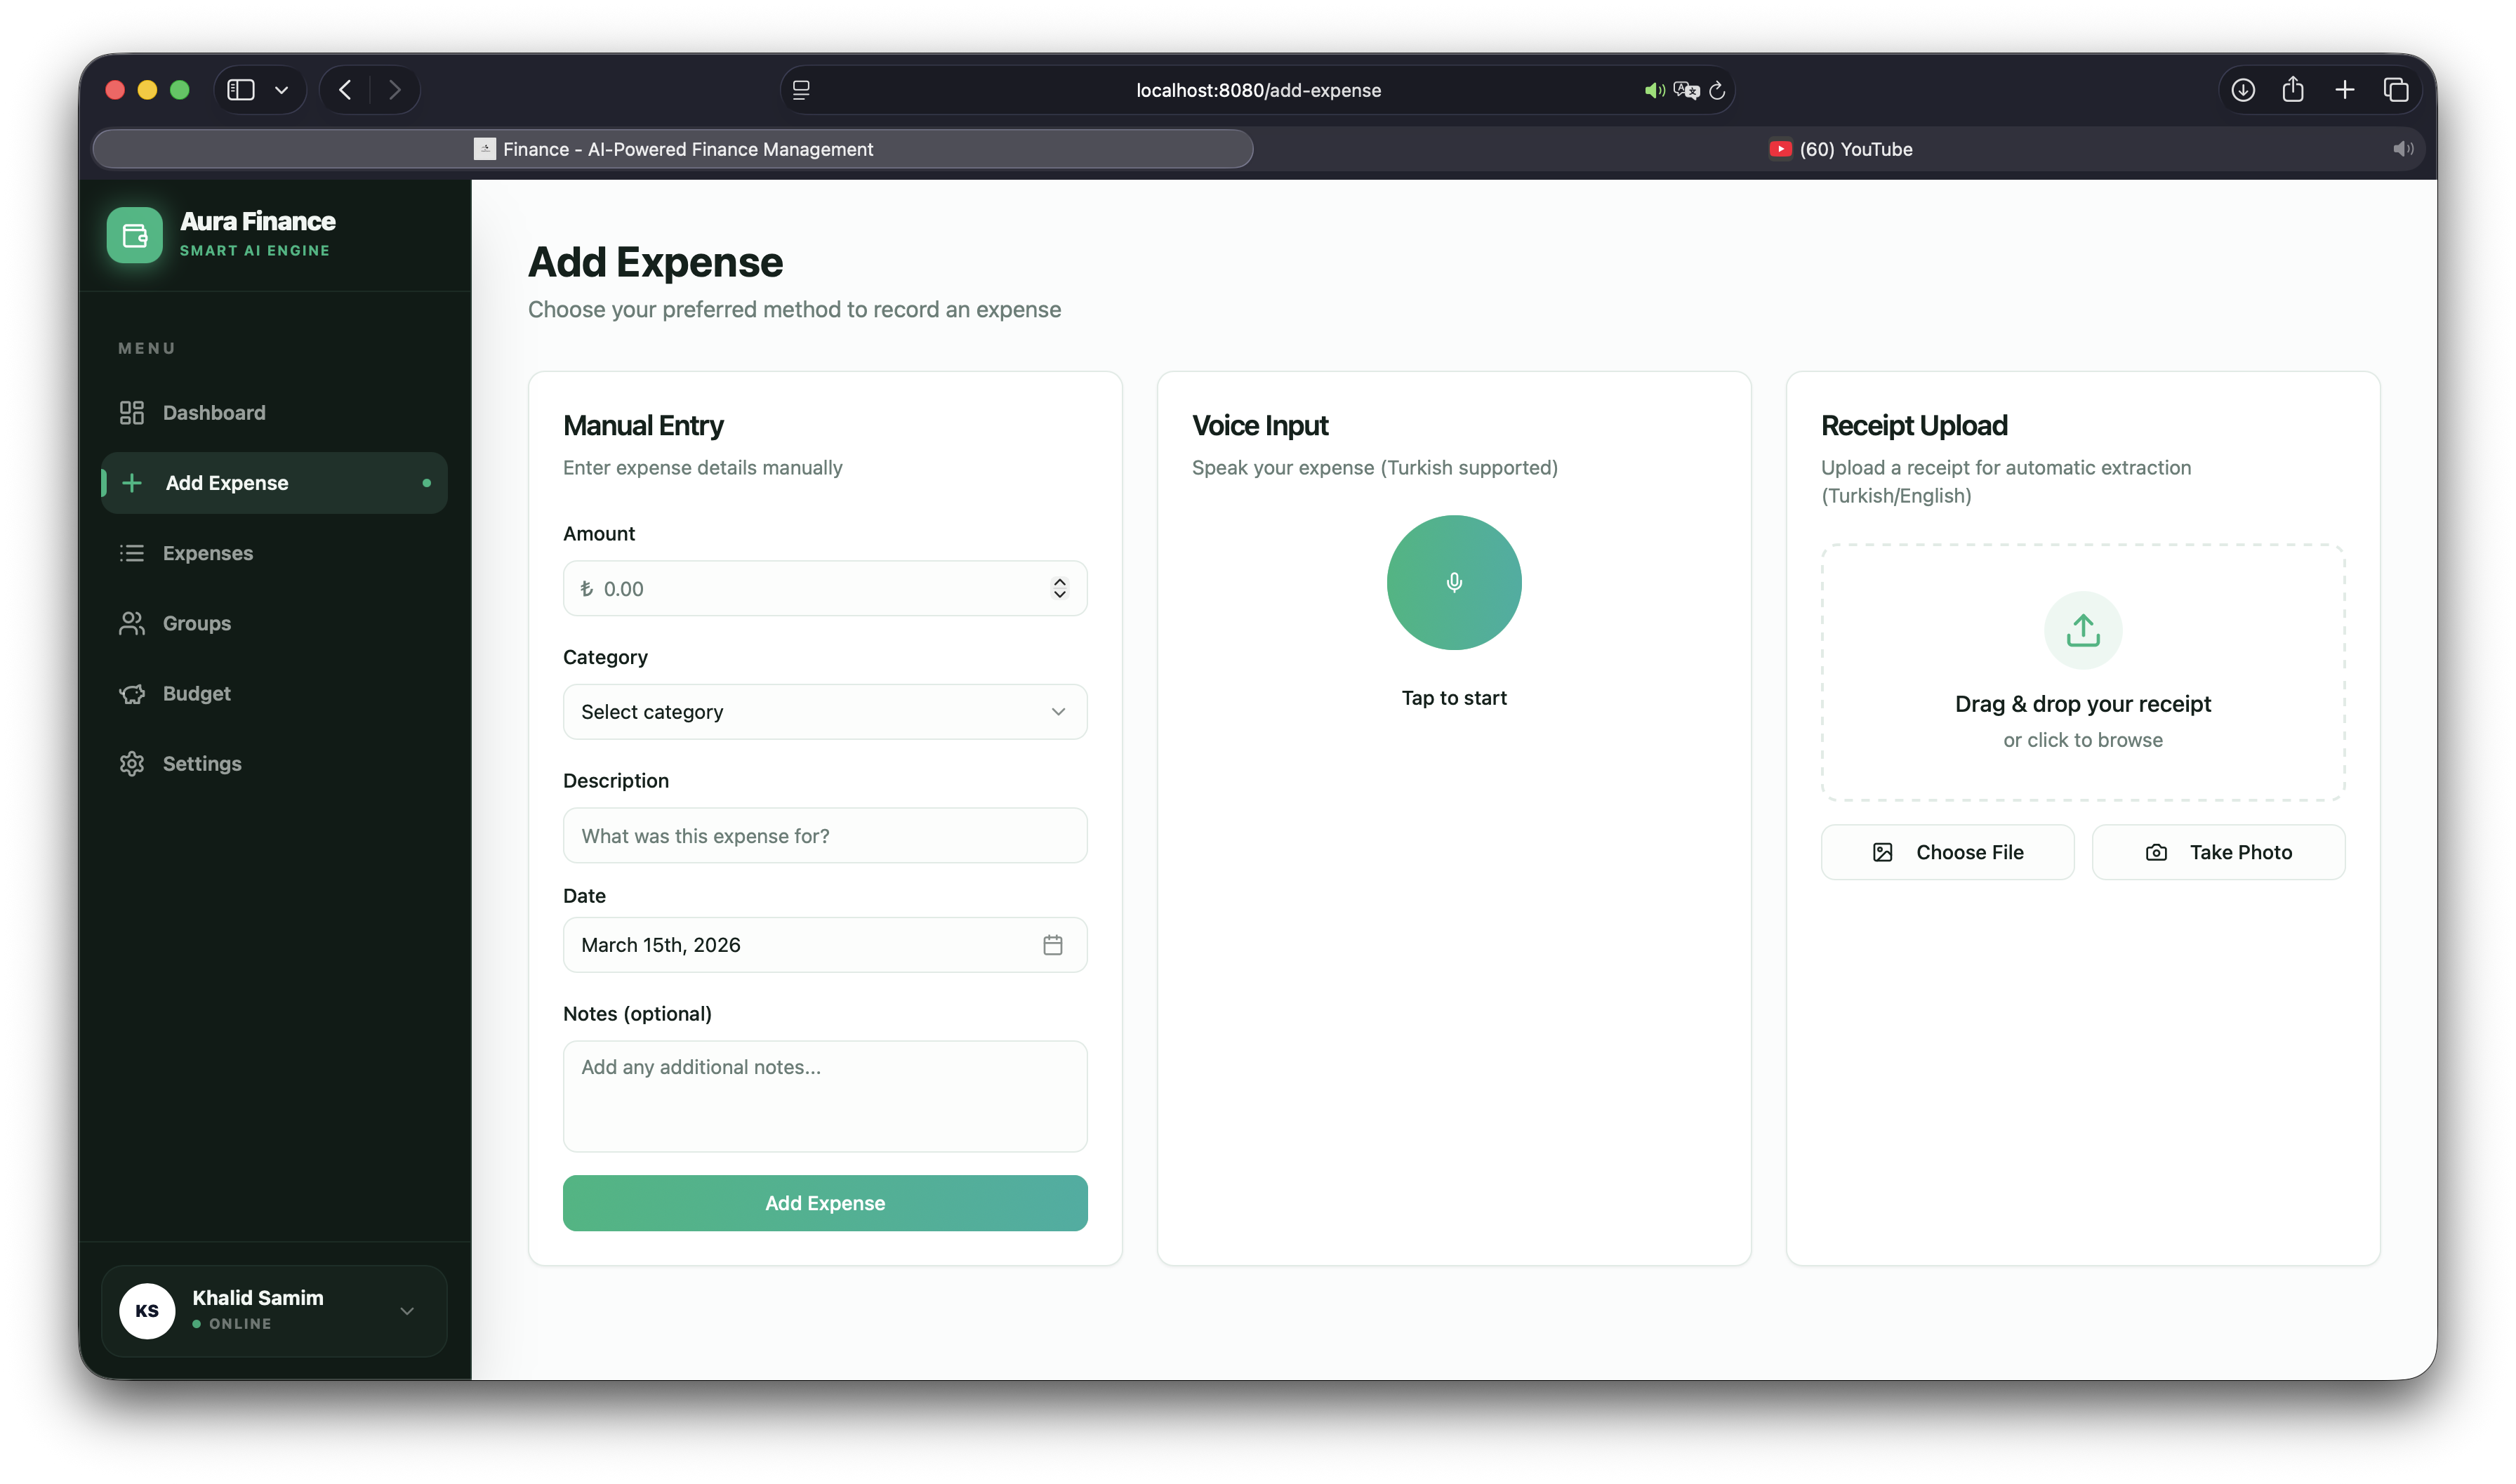
\includegraphics[width=0.6\textwidth]{./fig/aura_sc5}
 \caption{OCR ile Otomatik Makbuz Okuma ve Veri Ayrıştırma.}
 \label{fig:sc5}
\end{figure}

\begin{figure}[h!]
 \centering
 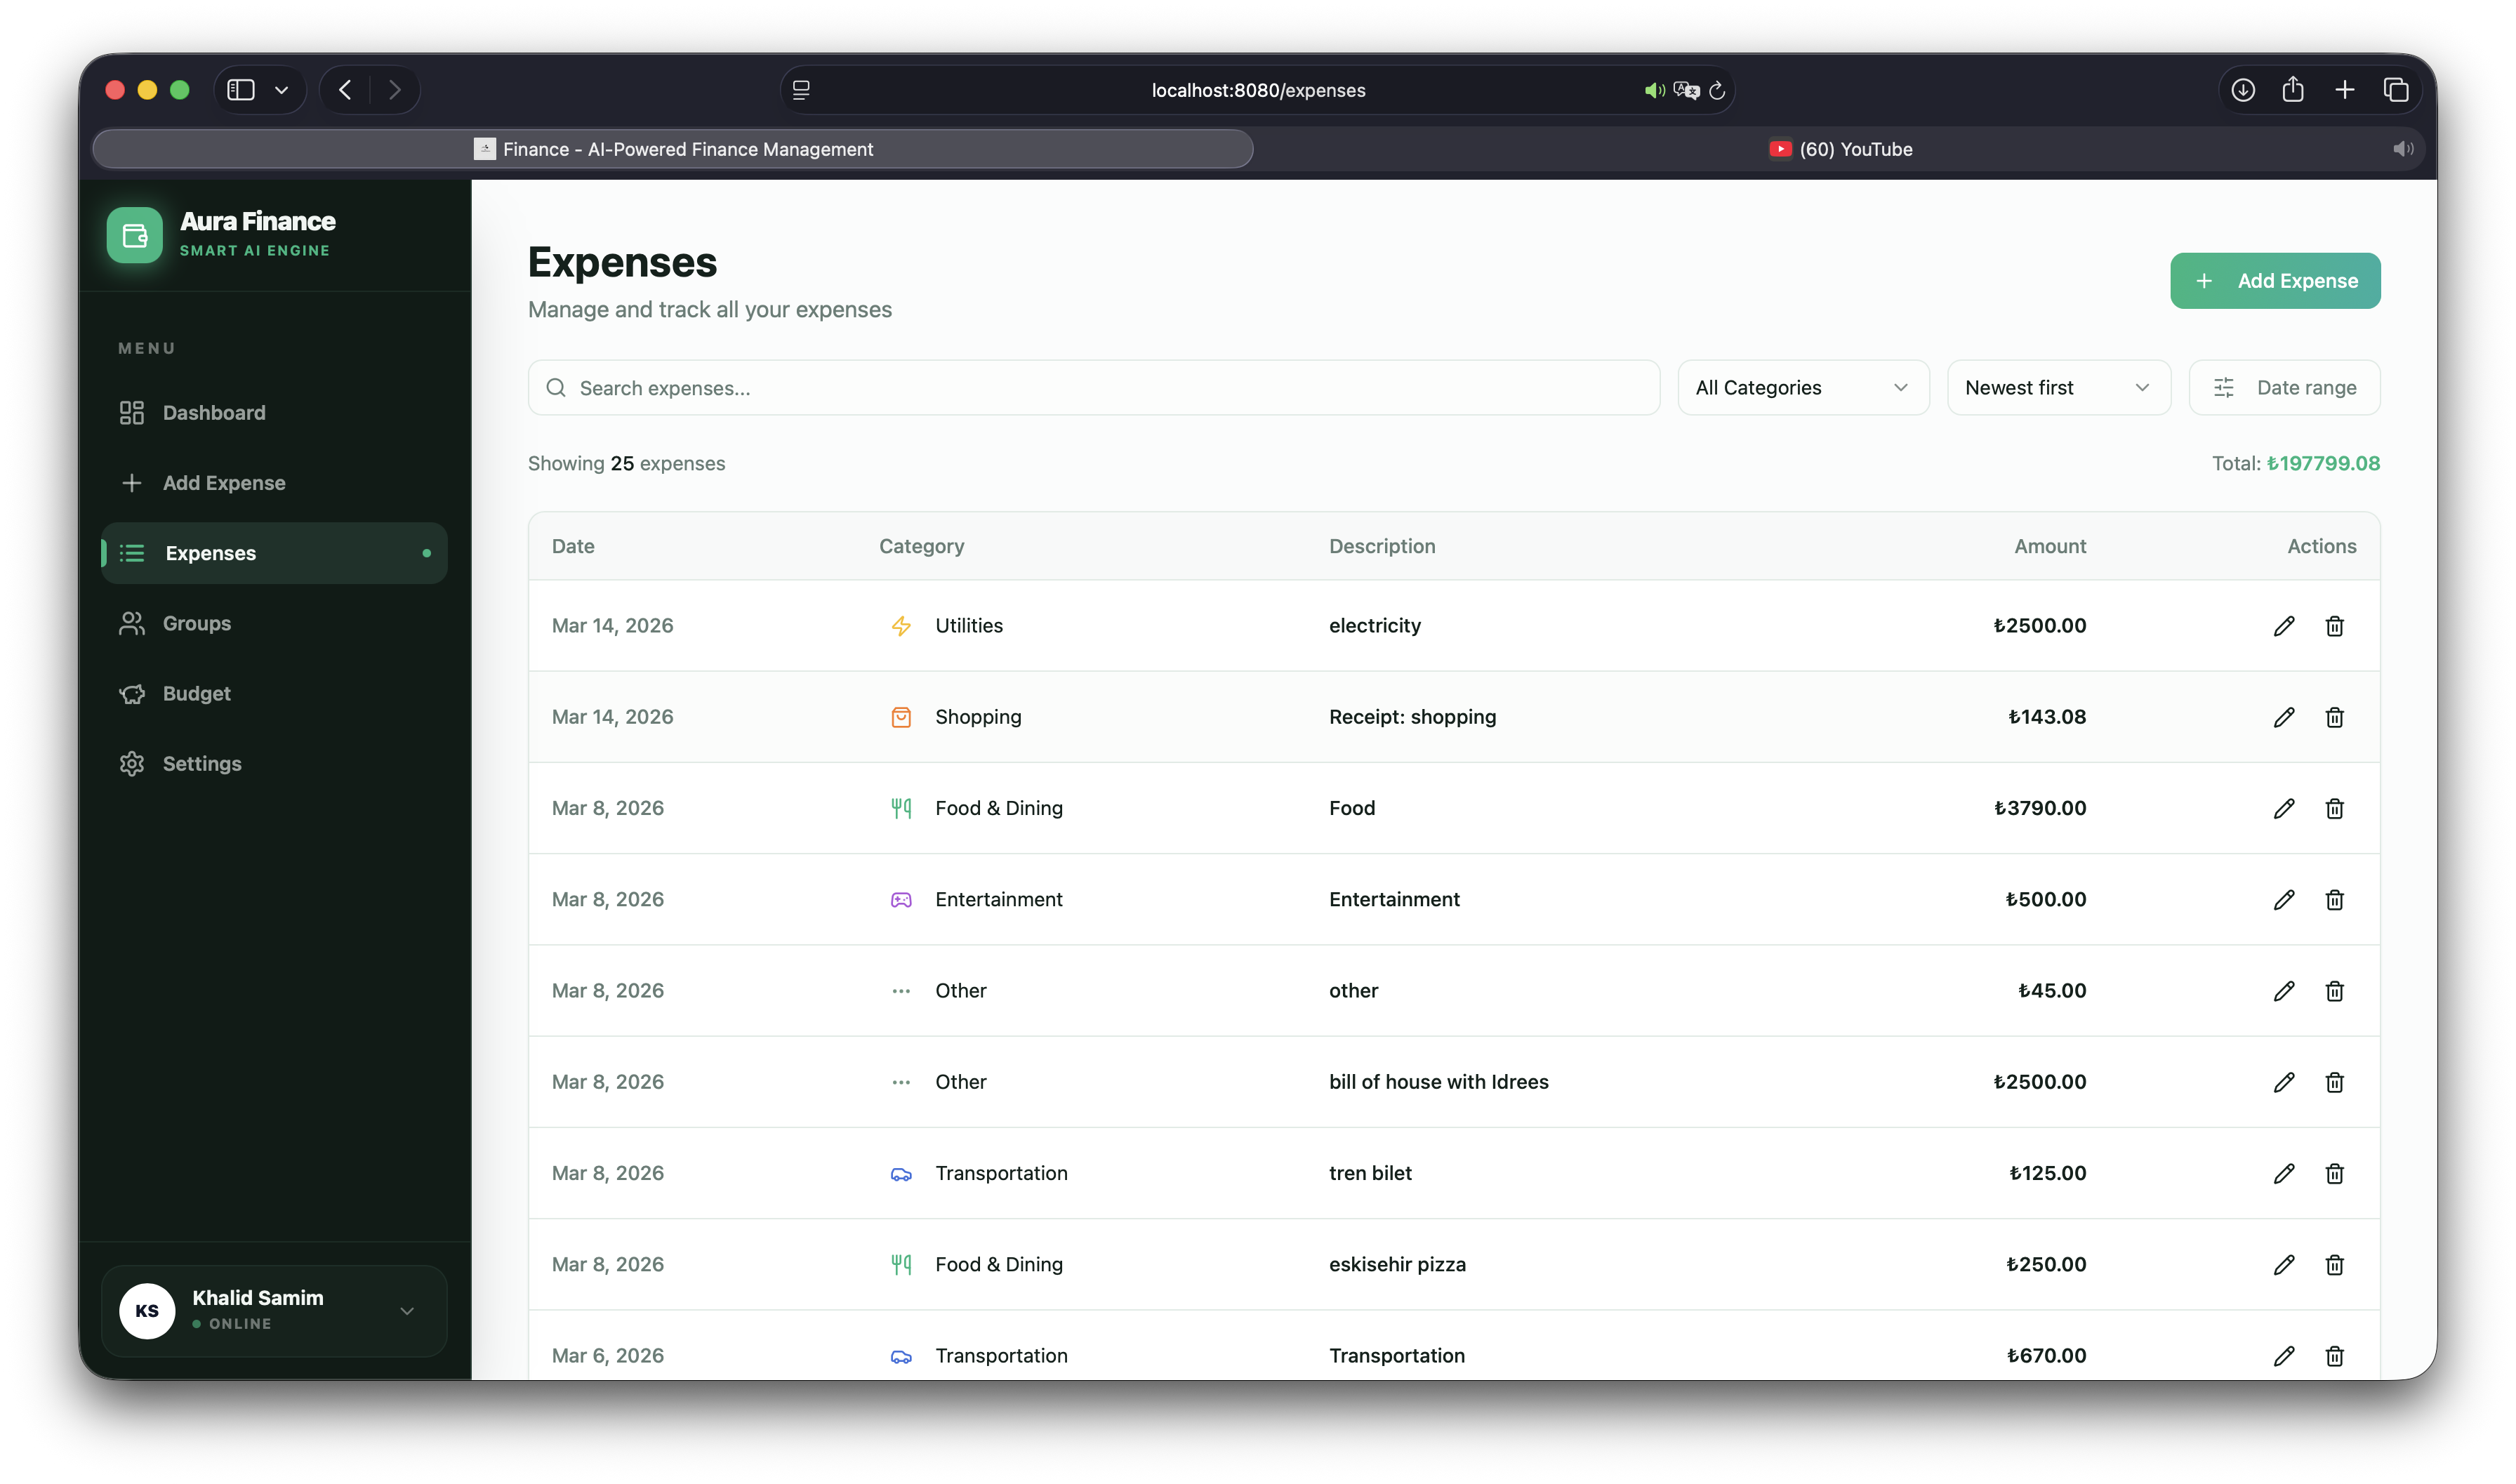
\includegraphics[width=0.8\textwidth]{./fig/aura_sc6}
 \caption{Grup Yönetimi: Yeni Grup Oluşturma Arayüzü.}
 \label{fig:sc6}
\end{figure}

\begin{figure}[h!]
 \centering
 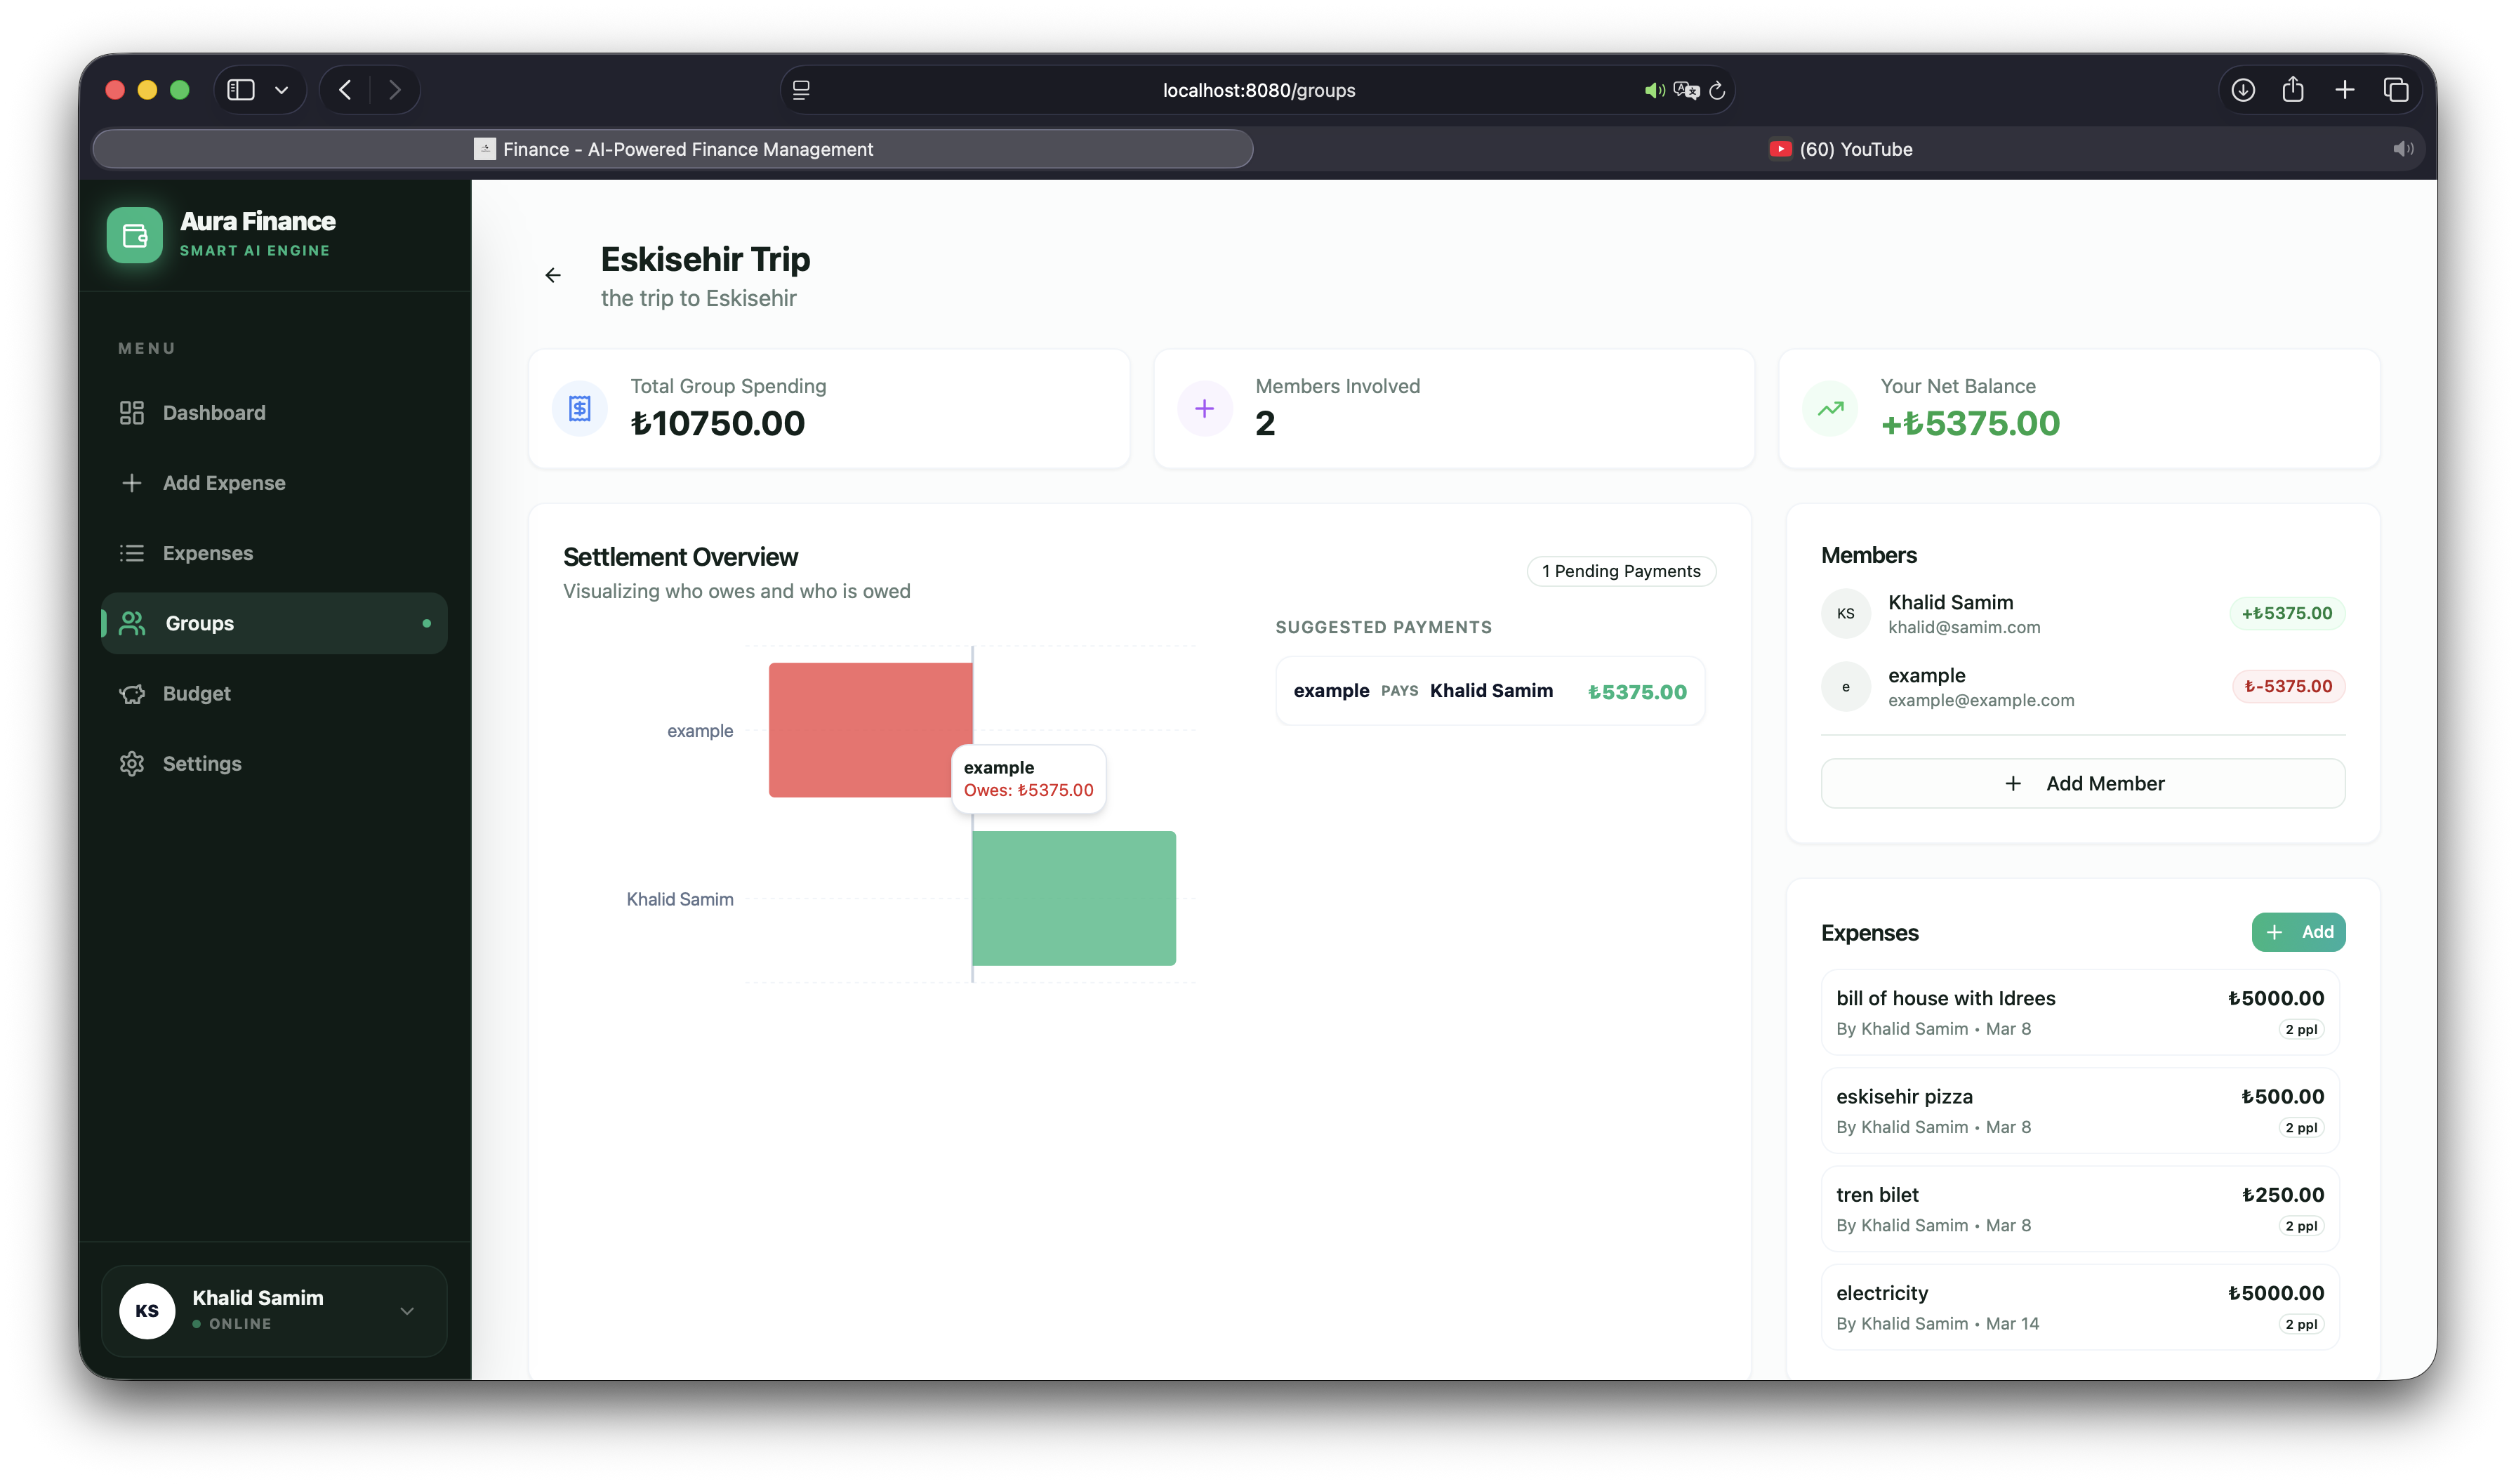
\includegraphics[label=sc7, width=0.8\textwidth]{./fig/aura_sc7}
 \caption{Grup Harcamaları ve Adil Paylaşım Takibi.}
 \label{fig:sc7}
\end{figure}

\begin{figure}[h!]
 \centering
 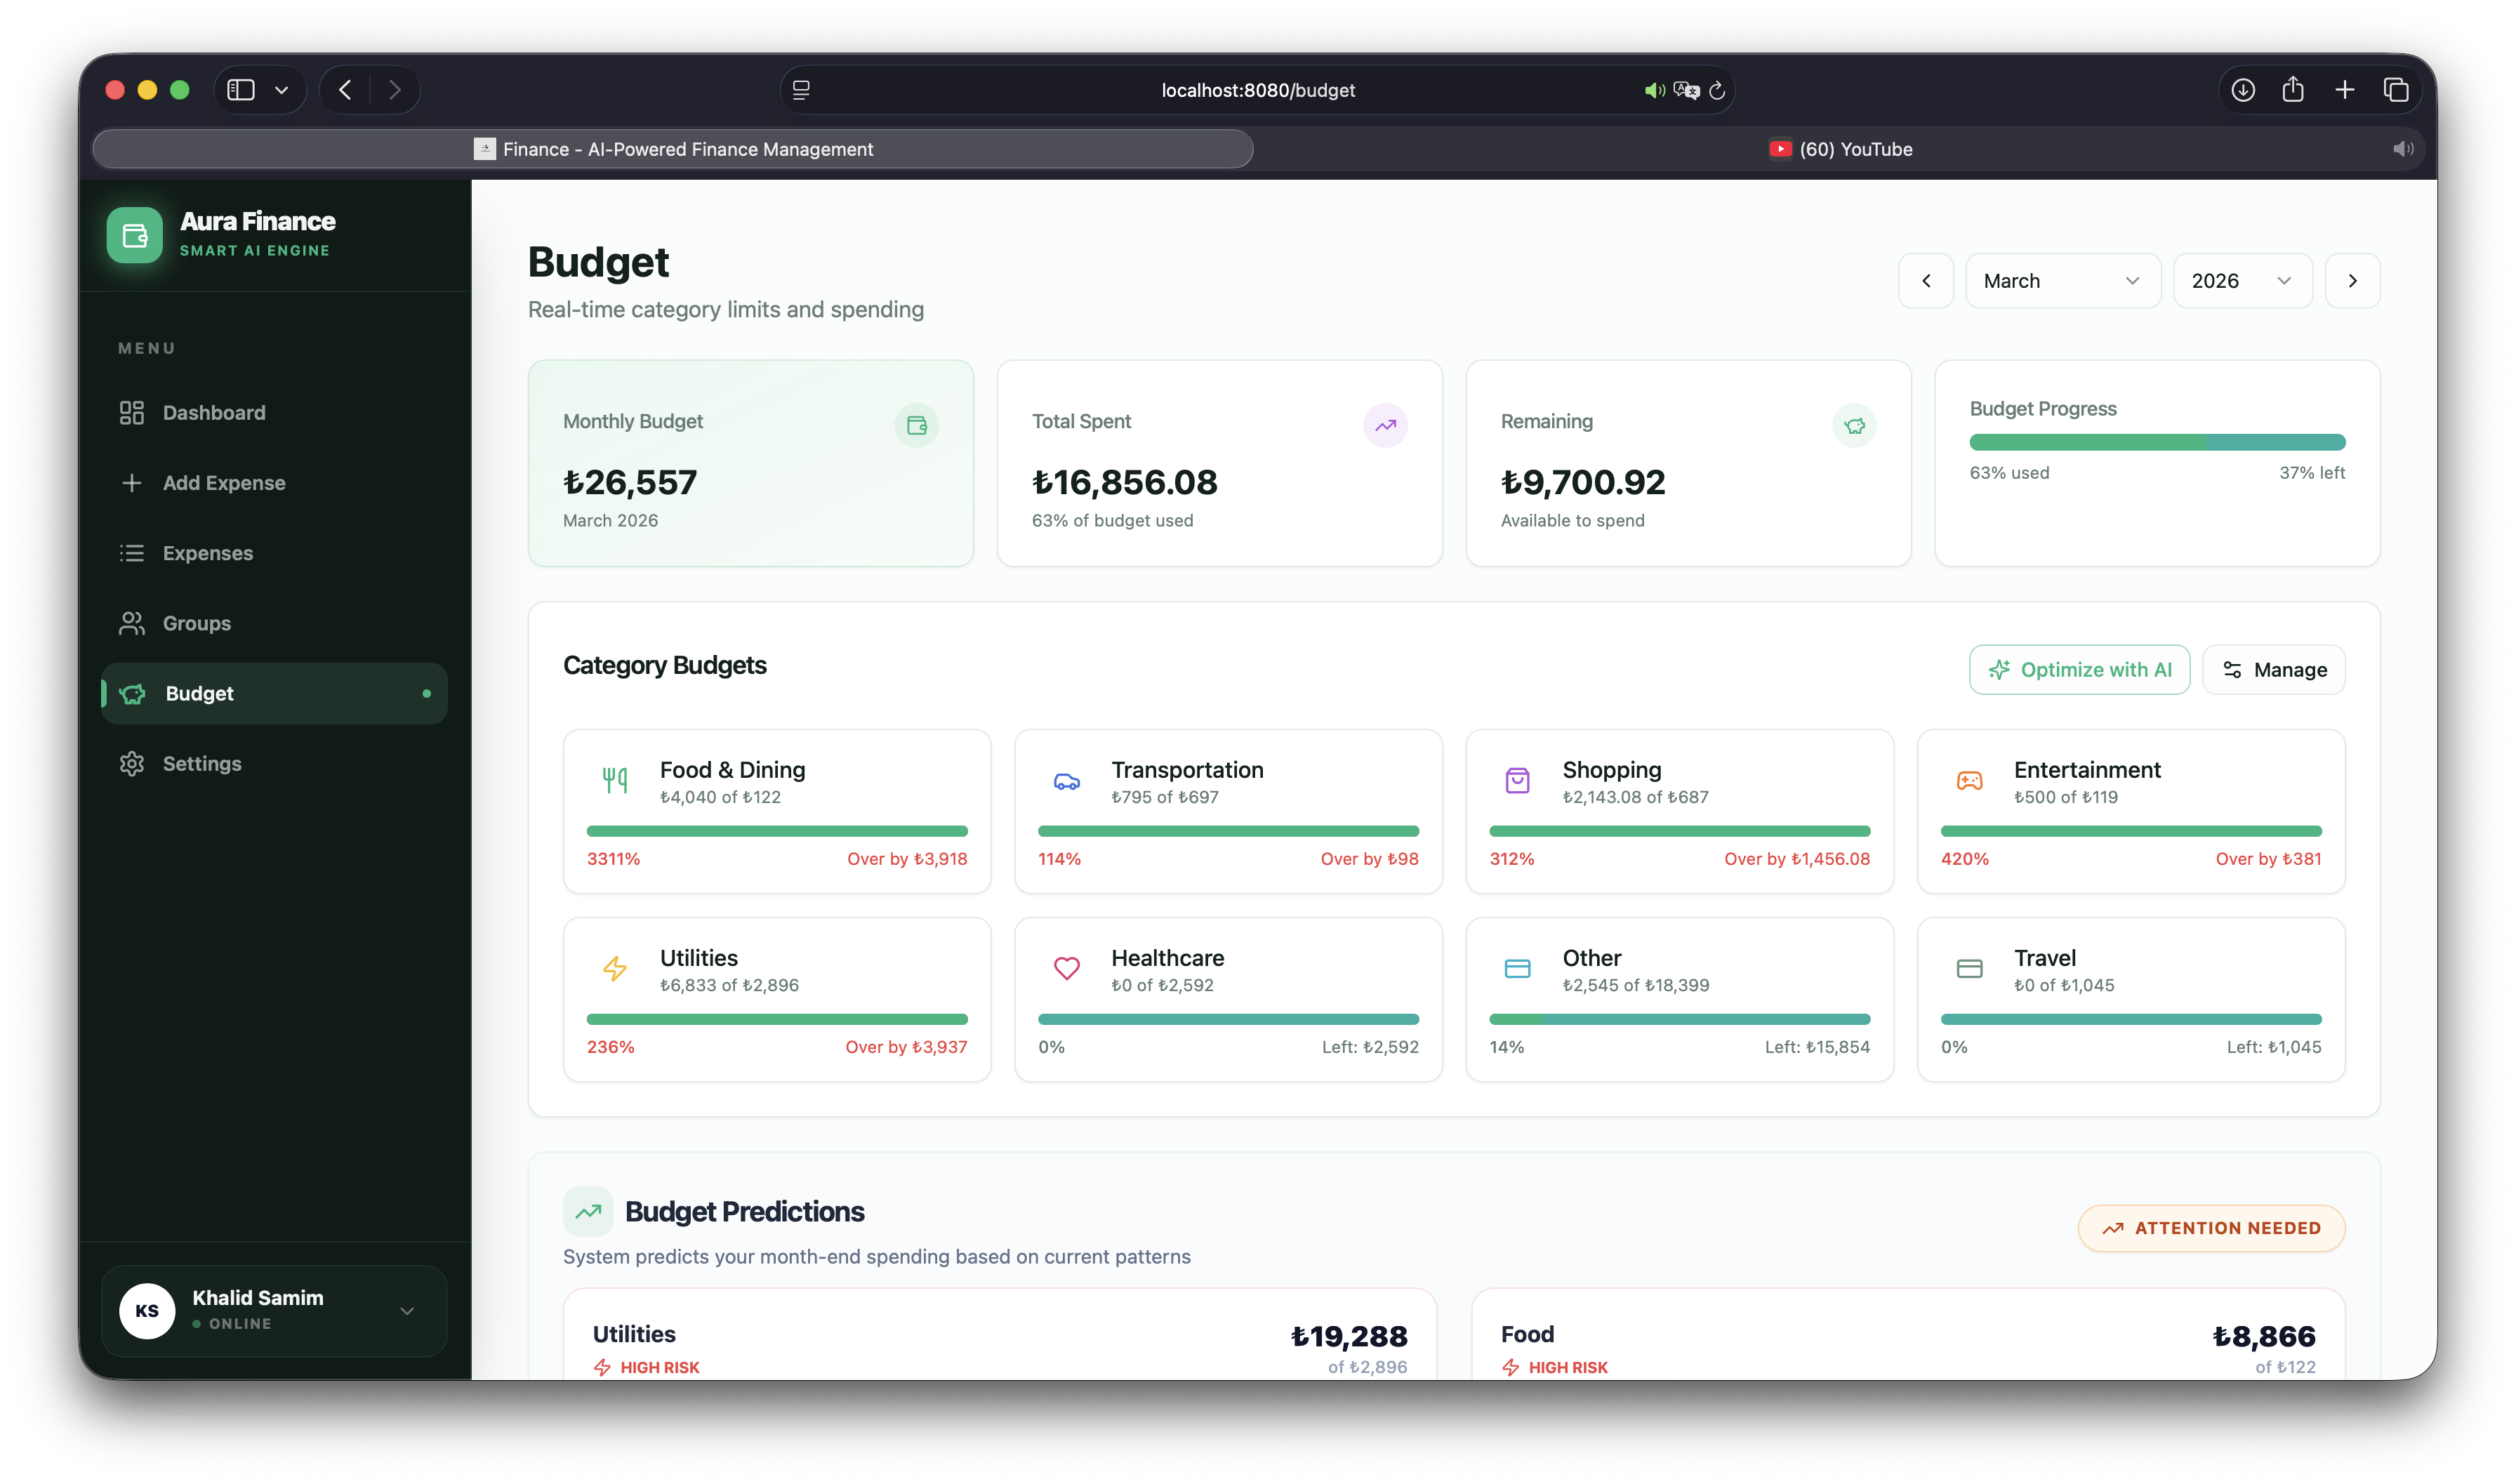
\includegraphics[width=0.8\textwidth]{./fig/aura_sc8}
 \caption{Ayarlar ve Kullanıcı Profili Yönetimi.}
 \label{fig:sc8}
\end{figure}

\clearpage

\input{sonuc}
\clearpage

\addcontentsline{toc}{chapter}{KAYNAKÇA}
\nocite{*}
\bibliographystyle{ieeetr}
\bibliography{references}

\end{document}
